\documentclass[11pt]{article}
\usepackage[margin=1in]{geometry}
\usepackage{setspace}
\usepackage{amsmath,amssymb}
\usepackage{graphicx}
\usepackage{booktabs}
\usepackage{array}
\usepackage{tabularx}
\usepackage{xurl}
\usepackage{float}
\usepackage{caption}
\usepackage{algorithm}
\usepackage{algpseudocode}
\usepackage{etoolbox}
\usepackage[hidelinks]{hyperref}

\setstretch{1.10}
\AtBeginEnvironment{algorithmic}{\setstretch{1.0}}
\AtBeginEnvironment{tabular}{\setstretch{1.0}}
\captionsetup{font=small,skip=4pt}
\setlength{\textfloatsep}{8pt}
\setlength{\intextsep}{6pt}
\setlength{\floatsep}{6pt}
\setlength{\abovedisplayskip}{7pt}
\setlength{\belowdisplayskip}{7pt}

% Advantages and limitations of one approach.
\newcommand{\proscons}[3]{%
\par\smallskip\noindent{\footnotesize
\begin{tabular}{|p{0.455\linewidth}|p{0.455\linewidth}|}
\hline
\textbf{Advantages of #3} & \textbf{Limitations of #3} \\
\hline
#1 & #2 \\
\hline
\end{tabular}}\par\smallskip}

\title{\textbf{Adaptive Data-Rate Control for Underwater Acoustic Networks}\\[4pt]
\large Final Report}
\date{November 2, 2026}

\begin{document}
\maketitle

\section*{Team Members}
\noindent\small
\begin{tabularx}{\linewidth}{@{}l l X@{}}
1. & 241CS132, M. Dhakshesh Naidu & \href{mailto:madakkagaridhaksheshnaidu.241cs132@nitk.edu.in}{\nolinkurl{madakkagaridhaksheshnaidu.241cs132@nitk.edu.in}} \\
2. & 241CS142, Pratham M. Attavar & \href{mailto:prathammattavar.241cs142@nitk.edu.in}{\nolinkurl{prathammattavar.241cs142@nitk.edu.in}} \\
3. & 241CS158, Srikara Nikhil & \href{mailto:srikaranikhil.241cs158@nitk.edu.in}{\nolinkurl{srikaranikhil.241cs158@nitk.edu.in}}
\end{tabularx}
\normalsize

\section*{Abstract}
\noindent
Underwater acoustic networks have long propagation delays, limited bandwidth, and packet loss~\cite{akyildiz2005,casari2011}.
A fixed application sending interval cannot use measured network conditions.
If the interval is too short, DATA frames and acknowledgment traffic can interfere.
If the interval is too long, the channel can stay unused.
We implemented an application-layer adaptive data-rate protocol in UnetStack~7.0.0~\cite{chitre2014,unethandbook}.
The fixed baseline sends at a 3000~ms interval, requests an acknowledgment for each original message, and does not retry at the application layer.
Protocol~v3 uses ten-message feedback windows, two original acknowledgment requests per window, immutable receiver snapshots, and bounded selective retry.
Its controller gives a weight of 0.55 to confirmed loss and a weight of 0.15 each to round-trip time, acknowledgment failure, and timeout.
We compared fixed mode and Protocol~v3 with the same topology, channel, duration, payload, and random seeds.
The held-out evaluation has 80 runs.
At 15~m, useful throughput increased from 102.54 to 133.26~bit/s, and packet-delivery ratio increased from 60.08\% to 82.57\%.
At 1000~m, useful throughput increased from 106.52 to 132.12~bit/s, and packet-delivery ratio increased from 62.42\% to 81.68\%.
The paired throughput gains were 30.63\% and 24.30\%.
The paired reliability gains were 22.48 and 19.26 percentage points.
All four paired 95\% bootstrap intervals exclude zero.
These results apply to the declared simulation.
They do not show that throughput always increases with water depth.

%==========================================================
\clearpage
\section{Introduction}\label{sec:intro}

\subsection{Background}\label{sec:background}
\noindent
Underwater nodes use acoustic communication because radio signals do not support long underwater links.
Sound moves through water at approximately 1500~m/s.
This low speed produces long propagation delays.
Acoustic links also have limited bandwidth, distance-dependent attenuation, multipath, and time-varying loss~\cite{akyildiz2005,casari2011}.
These properties make traffic timing important at the network and application layers.

An application sends DATA at a selected interval.
The interval is the time between paced DATA opportunities.
It is not the physical data rate of the modem.
A short interval can increase the number of transmission opportunities.
It can also increase overlap between DATA frames, acknowledgments, and reports.
A long interval can reduce overlap.
It can also reduce useful throughput if the network can accept more traffic.

A fixed-rate sender does not change the interval.
This method is simple and repeatable.
It cannot use round-trip time, receiver delivery evidence, acknowledgment behavior, or timeout history.
An adaptive sender can use this feedback to select a future interval.
The feedback must be interpreted correctly.
A missing acknowledgment does not prove that the DATA frame was lost.
The DATA frame can arrive while its acknowledgment is delayed or lost.

Automatic Repeat reQuest uses acknowledgments and retransmission to recover missing data.
This method is common in reliable communication.
In an underwater network, each feedback cycle can take several seconds.
An acknowledgment for each DATA frame can use channel time that new DATA needs.
Repeated retransmissions can also add load during a poor condition~\cite{tan2007}.

\subsection{Challenges and issues}\label{sec:challenges}
\noindent
The controller must make a decision from delayed and incomplete observations.
It must also limit the traffic that it creates.
The main issues are as follows.

\begin{enumerate}\setlength{\itemsep}{2pt}
  \item Long propagation delay makes feedback old when it arrives.
  \item Limited bandwidth makes an acknowledgment for every DATA frame expensive.
  \item A timeout can mean DATA loss, acknowledgment loss, or late feedback.
  \item A retry can recover a message, but many retries can increase congestion.
  \item Duplicate deliveries must not count as new useful data.
  \item A fair experiment must keep all non-controller conditions equal.
\end{enumerate}

Useful throughput must count new application information.
It must not count every transmission attempt.
For this reason, each original message has one stable sequence identifier.
A retry keeps the same identifier.
The receiver counts the identifier one time, even if both attempts arrive.

\clearpage
\subsection{Existing approaches and their issues}\label{sec:existing}
\noindent
Fixed-rate transmission uses one interval for the complete run.
It gives a clear baseline, but it cannot react to a changed condition.
Multi-hop ARQ uses acknowledgments and retransmissions to improve reliability~\cite{tan2007}.
It can recover packets, but acknowledgment traffic and stop-and-wait delay can be costly underwater.

Guo, Liu, and Feng proposed adaptive transmission control for an underwater acoustic sensor network~\cite{guo2008}.
Their method uses topology and bit-error-rate feedback to assign transmission times in a tree.
It targets collision reduction and energy use.
It does not use the receiver-validated window protocol in this project.
Casari and Zorzi show that underwater protocol design must account for long delay, limited bandwidth, channel behavior, and energy use~\cite{casari2011}.

The progress-stage controller in this repository used an interval of 3000~ms at startup.
It reacted to individual acknowledgment and timeout events.
This event-level rule was useful as an early prototype.
It had two limits.
First, one missing acknowledgment could be treated as a DATA problem.
Second, a new event could change the interval before a stable observation window was complete.

\subsection{Problem statement}\label{sec:problem}
\noindent
Design and evaluate an application-layer protocol that improves useful throughput and packet-delivery ratio over a fixed 3000~ms sender.
Use sparse acknowledgments, receiver-validated delivery evidence, adaptive pacing, and bounded selective retry.
Keep the topology, channel, duration, payload, and random seed equal for each fixed-and-proposed pair.

\subsection{Objectives}\label{sec:objectives}
\begin{enumerate}\setlength{\itemsep}{2pt}
  \item Implement the fixed baseline and Protocol~v3 in UnetStack~7.0.0.
  \item Use receiver evidence to separate confirmed missing DATA from missing acknowledgment feedback.
  \item Measure useful throughput, packet-delivery ratio, loss, retries, round-trip time, and timeouts.
  \item Compare the protocols with paired held-out seeds at 15~m and 1000~m.
  \item Recreate the final graphs in MATLAB from validated CSV files.
\end{enumerate}

\subsection{Organization of the report}\label{sec:organization}
\noindent
Section~\ref{sec:lit} reviews the existing methods and identifies the research gap.
Section~\ref{sec:prop} gives Protocol~v3 and the reason for each design rule.
Section~\ref{sec:impl} explains the UnetStack implementation, class structure, and pseudocode.
Section~\ref{sec:results} gives the experiment design, metrics, numerical results, graphs, and comparison with the reviewed methods.
Section~\ref{sec:conclusion} gives the conclusion and future work.

%==========================================================
\clearpage
\section{Literature review}\label{sec:lit}
\noindent
This section reviews the methods in publication order.
The comparison focuses on feedback, traffic control, recovery, and measurement cost.

\subsection{Underwater acoustic sensor-network challenges (2005)}\label{sec:lit-akyildiz}
\noindent
Akyildiz, Pompili, and Melodia describe architectures and research challenges for underwater acoustic sensor networks~\cite{akyildiz2005}.
They identify long propagation delay, low bandwidth, high error rates, and energy limits as major design conditions.
They also explain that terrestrial network protocols cannot be moved underwater without changes.

Their work defines the problem context.
It does not give the application-layer controller in this project.
It shows why the controller must limit feedback and must account for long delay.

\proscons{Gives a complete description of underwater network constraints. Connects channel properties to protocol design.}
{It is a survey and architecture paper. It does not give a receiver-validated rate controller.}
{the underwater-network survey}

\subsection{Multi-hop ARQ (2007)}\label{sec:lit-arq}
\noindent
Tan, Seah, and Doyle proposed an opportunistic acknowledgment method for stop-and-wait ARQ in multi-hop underwater acoustic networks~\cite{tan2007}.
The method uses overheard acknowledgments to reduce the delay and energy cost of conventional hop-by-hop acknowledgment.
It shows that acknowledgment design has a large effect when propagation delay is long.

ARQ gives direct recovery, but it can create more transmissions when the channel is poor.
It also depends on acknowledgment delivery.
A lost acknowledgment can cause a retransmission even when the DATA frame arrived.
Protocol~v3 uses acknowledgments for sampled timing information and uses a receiver snapshot for delivery evidence.

\begin{algorithm}[H]
\caption{Stop-and-wait ARQ at one sender}\label{alg:arq}
\footnotesize
\begin{algorithmic}[1]
\Require DATA packet $P$, retry limit $R$
\Ensure Delivery acknowledgment or failure result
\State $r \gets 0$
\Repeat
  \State Send $P$ and start the ACK timer
  \If{the matching ACK arrives}
    \State \Return success
  \EndIf
  \State $r \gets r+1$
\Until{$r>R$}
\State \Return failure
\end{algorithmic}
\end{algorithm}

\proscons{Uses receiver feedback and can recover a missing packet. Opportunistic acknowledgment can reduce delay.}
{ACK traffic uses capacity. A lost ACK can cause an unnecessary retransmission. Stop-and-wait operation can be slow on a long-delay link.}
{multi-hop ARQ}

\clearpage
\subsection{Adaptive transmission control (2008)}\label{sec:lit-atc}
\noindent
Guo, Liu, and Feng proposed adaptive transmission control for an underwater acoustic sensor network~\cite{guo2008}.
Their network has a tree structure.
Nodes report topology and bit-error-rate information.
The sink uses this information to assign transmission times.
The method reduces collision and repeated transmission in the evaluated settings.

ATC shows that feedback can control underwater transmission time.
Its state and objective differ from this project.
ATC calculates a schedule for nodes in a tree and studies energy use.
Protocol~v3 controls the sending interval of an application flow and measures unique payload delivery.

\proscons{Adapts transmission time to topology and link quality. Targets collision and energy reduction.}
{Needs topology and bit-error-rate information. Uses a different network state, controller, and evaluation metric.}
{adaptive transmission control}

\subsection{Protocol design issues (2011)}\label{sec:lit-casari}
\noindent
Casari and Zorzi review protocol design for underwater acoustic networks~\cite{casari2011}.
They explain the effects of propagation speed, bandwidth, energy use, and channel modeling.
They also discuss scheduling, topology management, and hop-distance decisions.

Their analysis supports two design rules in this project.
First, the controller must keep feedback traffic small.
Second, simulation results depend on the declared channel model and geometry.
The paper does not give the exact feedback window, score, or retry scheduler used here.

\proscons{Connects underwater channel properties to protocol decisions. Explains why channel models and timing rules matter.}
{Does not define a project-specific application controller or a fixed-versus-adaptive experiment.}
{the protocol-design review}

\subsection{UnetStack (2014)}\label{sec:lit-unet}
\noindent
Chitre, Bhatnagar, and Soh describe UnetStack as an agent-based network stack and simulator~\cite{chitre2014}.
The agent model supports simulation and deployment on compatible modem platforms.
The stack exposes services and notifications that protocol agents can use.
The UnetStack handbook defines the simulator and ProtocolChannelModel interfaces~\cite{unethandbook}.

UnetStack is the central implementation tool in this project.
It supplies the network execution environment.
It does not select the application sending interval.
The proposed Groovy agents implement that decision.

\proscons{Supports repeatable network simulation and agent-based protocol code. The same agent model can support later modem deployment.}
{A simulation result still depends on the selected topology, model, probabilities, and run duration.}
{UnetStack}

\clearpage
\subsection{Progress-stage event controller}\label{sec:lit-legacy}
\noindent
The progress-stage prototype used ACK, RTT, and timeout events to change the interval after individual observations.
It increased the interval when delay or loss appeared high.
It decreased the interval when observations appeared healthy.
The interval stayed between configured minimum and maximum values.

This controller is the legacy adaptive controller in the repository.
It is not the fixed baseline.
The controller can react quickly, but one event can change its state.
It also has no immutable receiver snapshot for a completed window.
Protocol~v3 replaces per-event control with windowed evidence and bounded recovery.

\proscons{Simple feedback rule. Uses measured RTT and timeout events.}
{A missing ACK does not prove DATA loss. Per-event updates can react to incomplete or late observations.}
{the legacy controller}

\subsection{Comparison and research gap}\label{sec:lit-compare}
\noindent
Table~\ref{tab:lit-compare} compares the reviewed approaches.
The literature establishes the need for underwater-specific timing and feedback.
It does not give the complete protocol required for this project.
Three gaps remain.

\begin{enumerate}\setlength{\itemsep}{2pt}
  \item The fixed baseline cannot adapt.
  \item ACK-only control cannot always separate missing DATA from missing feedback.
  \item Unbounded or frequent recovery can increase traffic during a poor condition.
\end{enumerate}

\begin{table}[H]
\centering\footnotesize\setlength{\tabcolsep}{3pt}
\caption{Comparison of the reviewed approaches.}\label{tab:lit-compare}
\begin{tabular}{>{\raggedright\arraybackslash}p{2.7cm} >{\raggedright\arraybackslash}p{3.3cm} >{\raggedright\arraybackslash}p{3.4cm} >{\raggedright\arraybackslash}p{4.4cm}}
\toprule
Approach & Main feedback & Traffic action & Limit for this project \\
\midrule
Fixed rate & None for rate selection & Constant interval & Cannot react to observations \\
Multi-hop ARQ~\cite{tan2007} & ACK state & Retransmit packet & Feedback and retry cost \\
ATC~\cite{guo2008} & BER and topology & Assign transmission time & Different state and objective \\
Protocol guidance~\cite{akyildiz2005,casari2011} & Design principles & No single controller & No project-specific algorithm \\
Legacy controller & ACK, RTT, timeout & Per-event interval update & No receiver-validated window \\
\textbf{Protocol~v3} & Sparse ACK and receiver snapshot & Windowed interval and bounded retry & Requires receiver report state \\
\bottomrule
\end{tabular}
\end{table}

Protocol~v3 addresses these gaps.
It uses sparse acknowledgments, receiver-validated delivery evidence, one paced opportunity stream, and hard retry limits.

%==========================================================
\clearpage
\section{Proposed approach}\label{sec:prop}

\subsection{System model}\label{sec:prop-model}
\noindent
The simulation has three nodes.
Node~A is the sender.
Nodes~B and~C are receivers.
Node~A is at $(0\,\mathrm{km},0,-15\,\mathrm{m})$.
Node~B is at $(1\,\mathrm{km},0,-15\,\mathrm{m})$.
Node~C is at $(2\,\mathrm{km},0,-d)$, where $d$ is 15 or 1000~m.
The sender alternates destinations between B and C.

The modem data rate is 2400~bit/s.
Each application DATA payload is 64~bytes.
The channel uses the moderate scenario with detection probability 0.96 and decoding probability 0.94.
Each run has a 60~s warm-up, a 180~s measurement period, and a bounded drain period.

\subsection{Fixed baseline}\label{sec:prop-fixed}
\noindent
The fixed baseline uses a 3000~ms application sending interval.
It requests an acknowledgment for each original message.
It does not do an application-layer retry.
The fixed interval does not use RTT, confirmed loss, acknowledgment failure, or timeout observations.

\subsection{Protocol v3 overview}\label{sec:prop-v3}
\noindent
Protocol~v3 groups ten original messages into one source window.
It requests an ACK for the last two original positions in a full window.
Each retry requests an ACK.
The receiver stores unique sequence identifiers.
It reports an immutable snapshot for a completed receiver window.

The sender compares expected identifiers with delivered identifiers.
It puts only confirmed missing identifiers in a deterministic retry queue.
After four new originals, one retry can use the next paced opportunity.
The window can use at most three retries.
One identifier can use at most two attempts.

\begin{table}[H]
\centering\footnotesize
\caption{Protocol~v3 design rules.}\label{tab:v3-rules}
\begin{tabular}{>{\raggedright\arraybackslash}p{3.0cm} >{\raggedright\arraybackslash}p{5.2cm} >{\raggedright\arraybackslash}p{6.0cm}}
\toprule
Function & Rule & Reason \\
\midrule
Feedback window & 10 original messages & Use one stable observation unit \\
Original ACK policy & Last 2 originals in the window & Reduce reverse traffic \\
Delivery evidence & First valid receiver snapshot & Keep historical evidence stable \\
Retry selection & Confirmed missing identifiers only & Do not retry delivered DATA \\
Retry cadence & One opportunity after 4 new originals & Prevent a retry burst \\
Retry cap & At most 3 per source window & Bound recovery overhead \\
Per-ID cap & At most 2 attempts & Prevent repeated retransmission \\
Interval update & Latch one candidate for a full window & Prevent a mid-window change \\
\bottomrule
\end{tabular}
\end{table}

Figure~\ref{fig:protocol-flow} shows the sender decision path.
The diagram uses the same window, ACK, retry, and interval rules as Algorithm~\ref{alg:protocol-v3}.

\begin{figure}[!htbp]
\centering
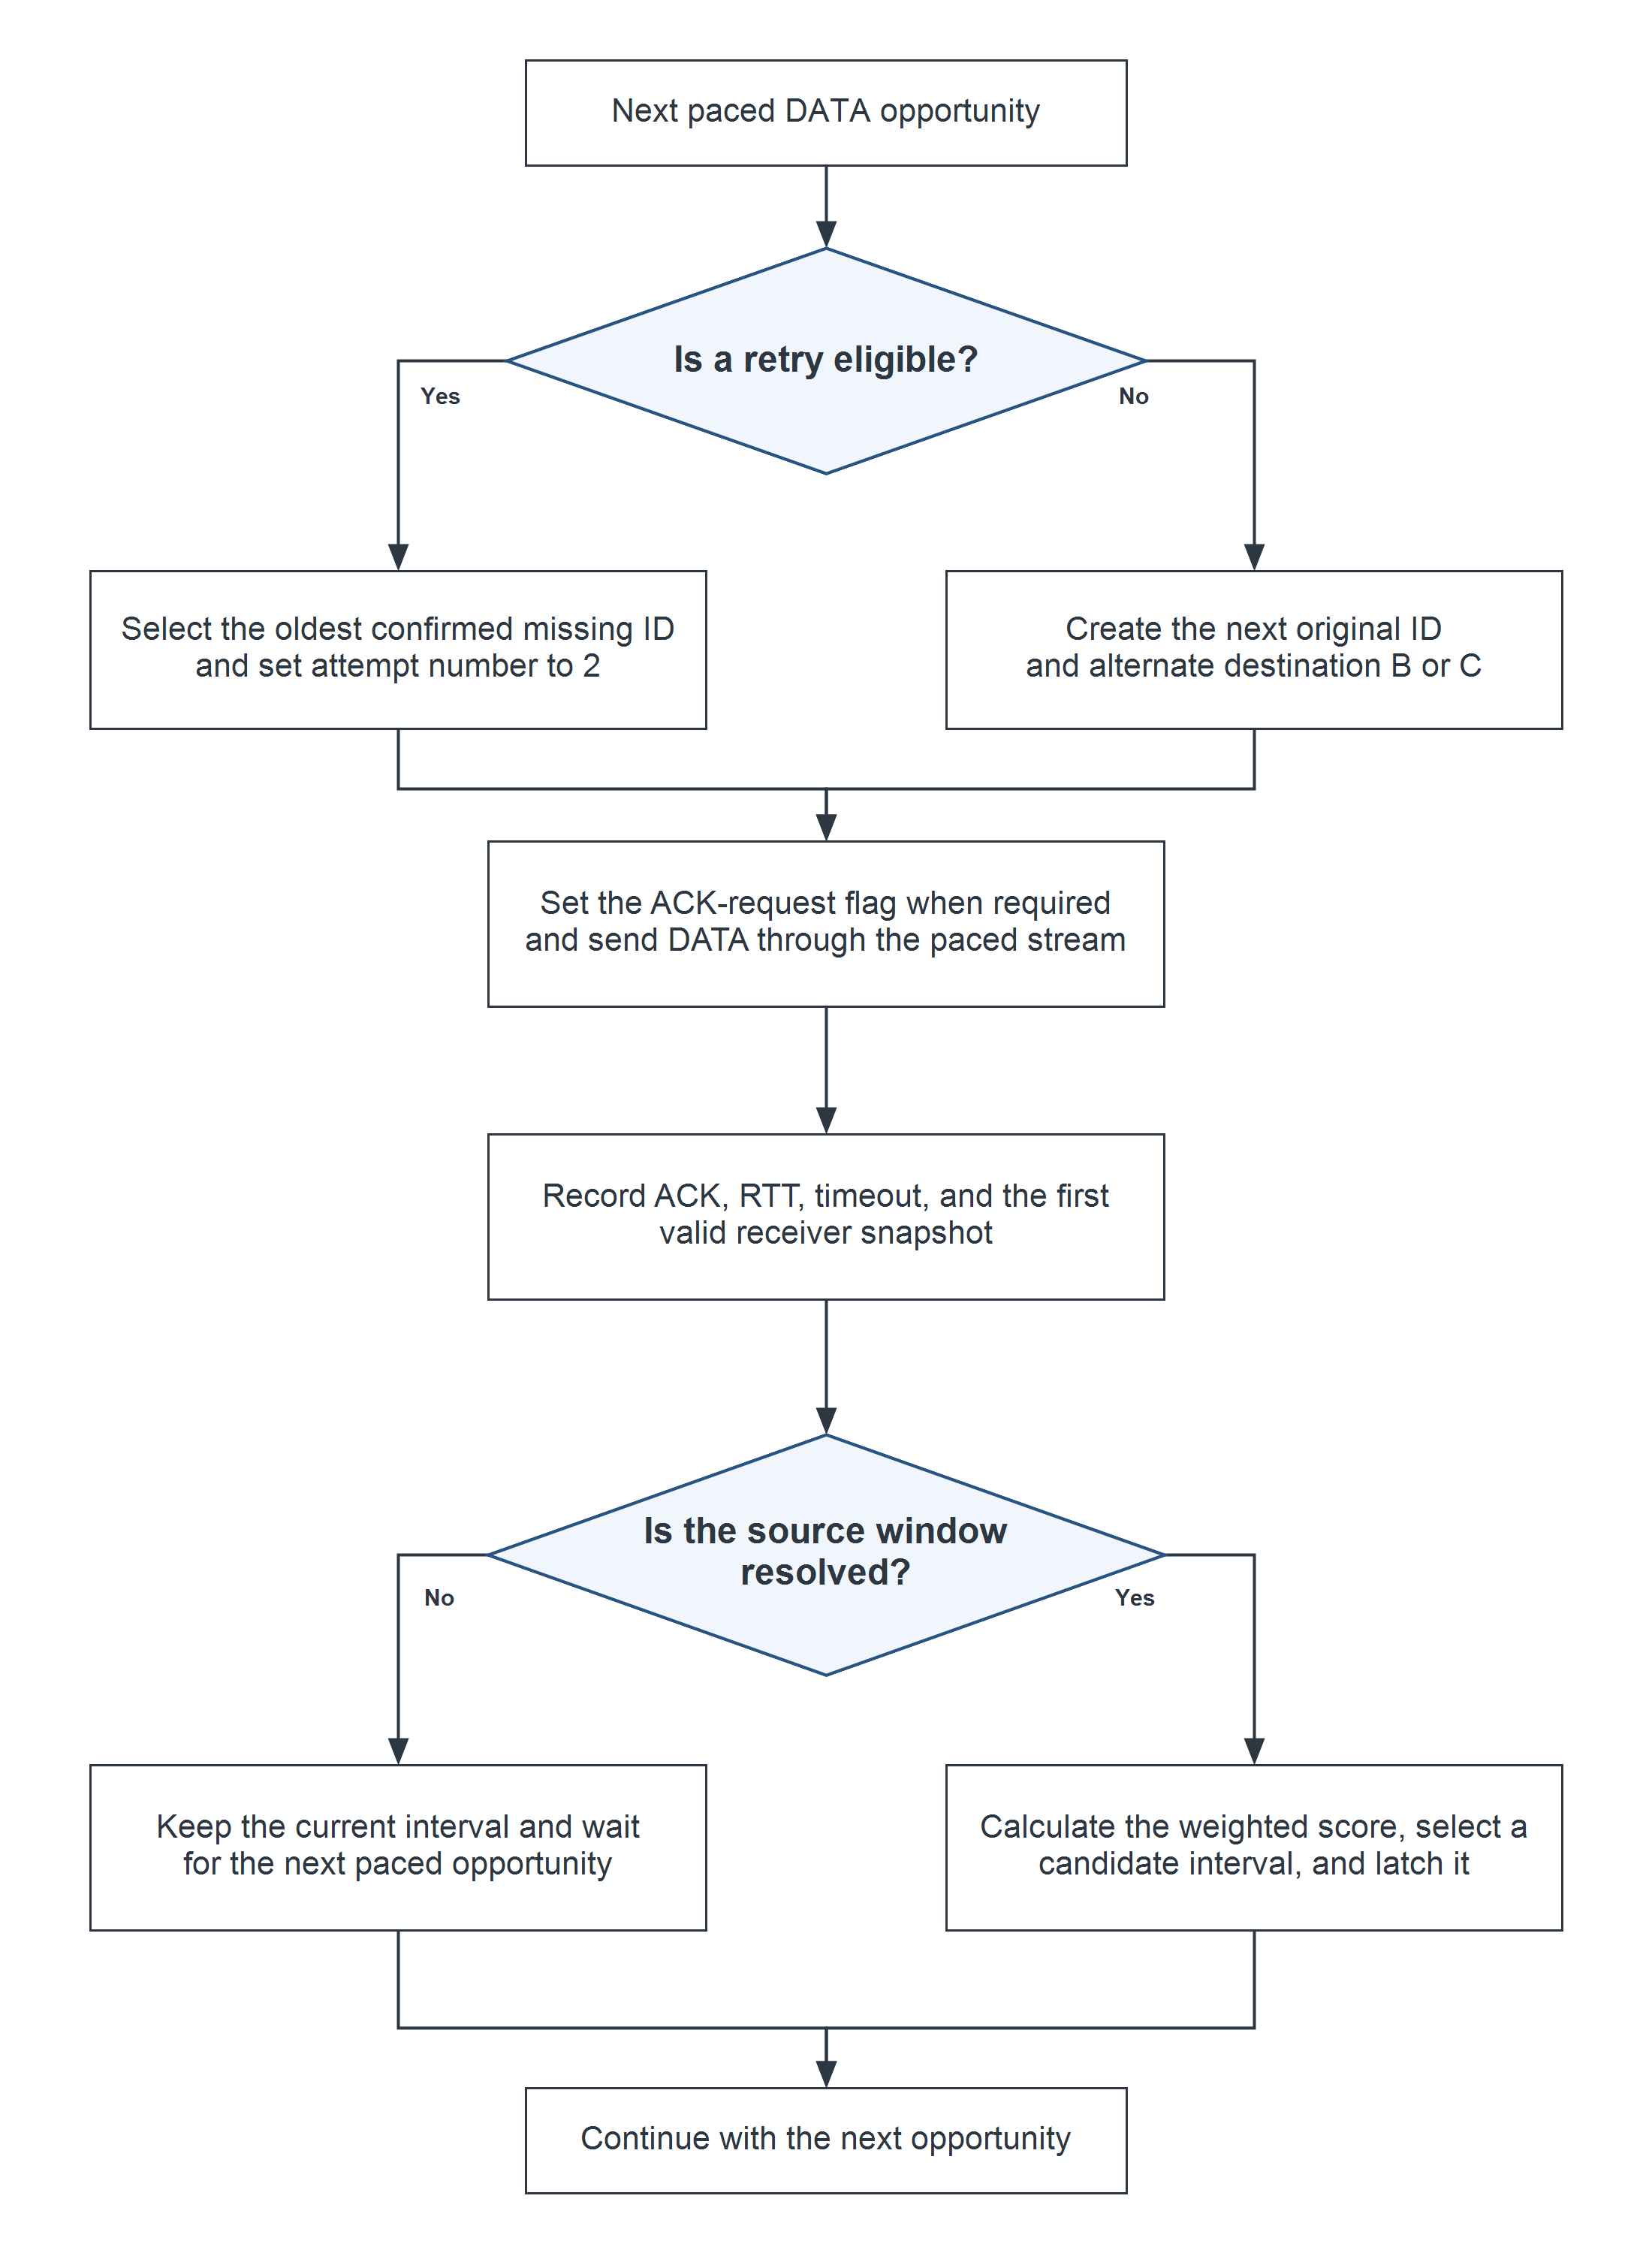
\includegraphics[height=0.76\textheight,width=0.98\linewidth,keepaspectratio]{images/protocol_flowchart.png}
\caption{Protocol~v3 sender flow. A retry is eligible only after receiver-confirmed loss, the four-original cadence, and the retry caps permit it.}\label{fig:protocol-flow}
\end{figure}

\subsection{Controller score}\label{sec:prop-score}
\noindent
The controller converts four observations to penalties between 0 and 1.
It calculates the score
\begin{equation}
S=0.15P_{\mathrm{RTT}}+0.55P_{\mathrm{loss}}+0.15P_{\mathrm{ACK}}+0.15P_{\mathrm{timeout}}.
\label{eq:score}
\end{equation}
Confirmed loss gets the largest weight because the receiver snapshot gives direct evidence of missing unique messages.
RTT, acknowledgment failure, and timeout remain useful warning signals.
A timeout does not prove DATA loss.

The controller selects the next interval from
\[
\{2000,2250,2500,2700,3000,3375,3750,4500,6000\}\ \mathrm{ms}.
\]
It latches the selected interval for the next complete source window.

\subsection{Sender algorithm}\label{sec:prop-algorithm}
\noindent
Algorithm~\ref{alg:protocol-v3} gives the complete sender sequence.
The algorithm uses one paced opportunity stream for originals and retries.

\begin{algorithm}[H]
\caption{Protocol~v3 sender}\label{alg:protocol-v3}
\footnotesize
\begin{algorithmic}[1]
\Require Fixed configuration, candidate intervals, receiver reports
\Ensure Event log, unique deliveries, and next-window intervals
\State Set the current interval to 3000~ms
\While{the measurement period is active}
  \State Create the next unique sequence identifier
  \State Select B or C with the alternating destination rule
  \If{the original is in one of the last two positions of its window}
    \State Request an ACK
  \EndIf
  \State Send the selected original through the paced stream
  \State Record ACK, RTT, timeout, and receiver-report events
  \If{the first valid snapshot for a completed receiver window arrives}
    \State Freeze the snapshot
    \State Queue each confirmed missing identifier
  \EndIf
  \If{four new originals occurred and an eligible retry exists}
    \State Use the next paced opportunity for one retry
  \EndIf
  \If{the source window is resolved}
    \State Calculate the weighted score in Equation~\ref{eq:score}
    \State Select and latch the next candidate interval
  \EndIf
\EndWhile
\end{algorithmic}
\end{algorithm}

\subsection{Why the method is an improvement}\label{sec:prop-justification}
\noindent
Sparse acknowledgments reduce reverse-channel traffic.
Receiver snapshots separate confirmed missing DATA from missing feedback.
Selective retry uses an opportunity only for an identifier that the receiver did not report.
The retry cadence mixes recovery with new traffic.
The hard caps prevent an uncontrolled retry loop.
Unique-message accounting prevents a duplicate from increasing useful throughput.

The method also improves the progress-stage legacy controller.
The legacy controller reacts to individual ACK and timeout events.
Protocol~v3 waits for a complete window and uses receiver-validated evidence.
The final held-out claim compares fixed mode with Protocol~v3.

\subsection{Metric integrity}\label{sec:prop-integrity}
\noindent
Each original message has one stable sequence identifier.
Attempt~1 is the original.
Attempt~2 is the only permitted retry.
If both attempts arrive, the receiver counts one unique delivery.
This rule prevents recovery traffic from manufacturing a throughput gain.

%==========================================================
\section{Implementation}\label{sec:impl}

\subsection{Tools and environment}\label{sec:impl-tools}
\noindent
We implemented the protocol in the UnetStack~7.0.0 community distribution.
The protocol agents and setup scripts use Groovy.
Python creates paired run matrices, validates manifests, and calculates the statistics.
MATLAB reads the validated summary CSV files and exports the final figures.

\begin{table}[H]
\centering\small
\caption{Implementation tools.}\label{tab:tools}
\begin{tabular}{p{4.2cm} p{10.2cm}}
\toprule
Item & Use in the project \\
\midrule
UnetStack~7.0.0 & Network stack, discrete-event simulation, services, and channel model \\
Groovy & Protocol agents, controller state, retry scheduler, setup, and experiment entry point \\
Python & Run matrix, manifest validation, metric calculation, paired bootstrap analysis \\
MATLAB R2026b & Final graphs from validated summary CSV files \\
\bottomrule
\end{tabular}
\end{table}

\subsection{Class diagram}\label{sec:impl-class}
\noindent
Figure~\ref{fig:class} shows the main classes.
The experiment entry point configures the network.
The agent uses the codec, state, scheduler, and controller during each run.

\begin{figure}[!htbp]
\centering
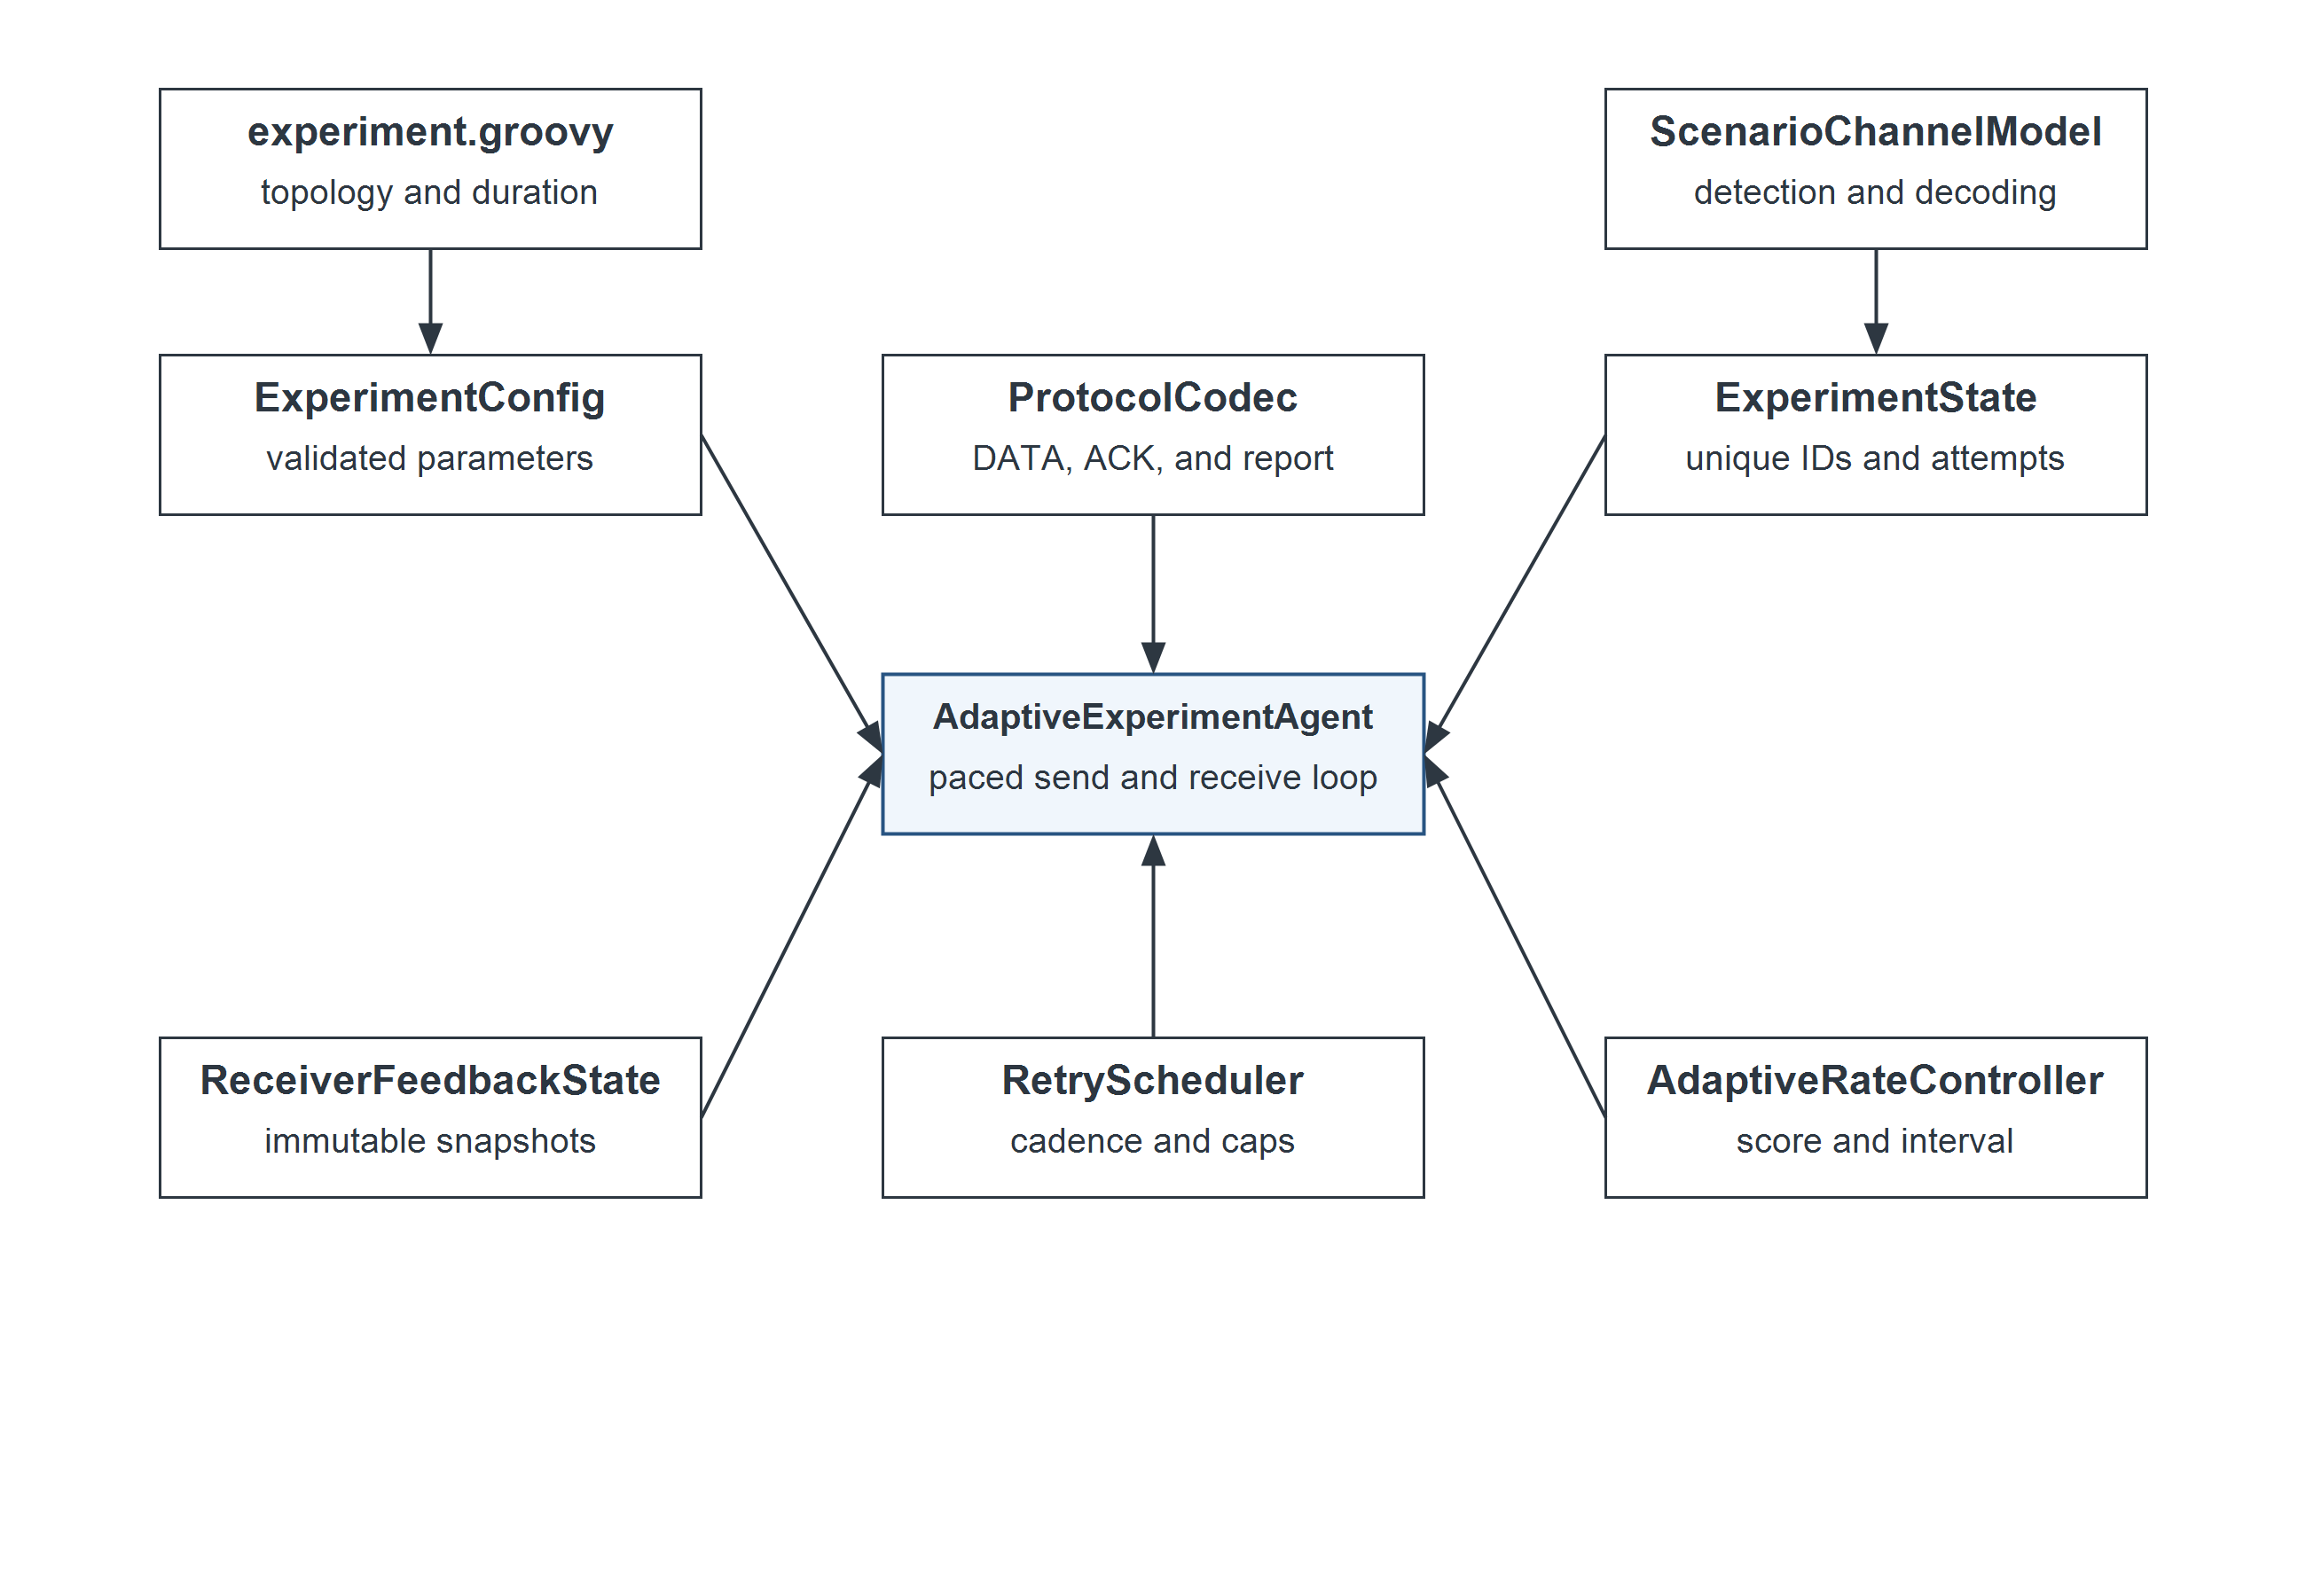
\includegraphics[width=0.98\linewidth]{images/class_diagram.png}
\caption{Class diagram of the Protocol~v3 implementation. Solid arrows show direct use. The dashed arrows show experiment and channel inputs to agent behavior.}\label{fig:class}
\end{figure}

\subsection{Source files}\label{sec:impl-files}
\begin{table}[!htbp]
\centering\small
\caption{Main source files and responsibilities.}\label{tab:files}
\renewcommand{\arraystretch}{1.12}
\begin{tabularx}{\linewidth}{>{\raggedright\arraybackslash}p{5.7cm} >{\raggedright\arraybackslash}X}
\toprule
File & Responsibility \\
\midrule
\path{simulations/experiment.groovy} & Configure channel, modem, topology, duration, and run manifest \\
\path{classes/ExperimentConfig.groovy} & Read and validate environment variables \\
\path{classes/ProtocolCodec.groovy} & Encode and decode DATA, ACK, report request, and receiver report \\
\path{classes/ExperimentState.groovy} & Store unique identifiers and attempts \\
\path{classes/ReceiverFeedbackState.groovy} & Store delivery state and create immutable snapshots \\
\path{classes/RetryScheduler.groovy} & Apply ACK policy, retry cadence, caps, and interval latch \\
\path{classes/AdaptiveRateController.groovy} & Calculate penalties, score, and candidate interval \\
\path{classes/AdaptiveExperimentAgent.groovy} & Send, receive, time, report, and log protocol events \\
\path{classes/ScenarioChannelModel.groovy} & Set scenario detection and decoding probabilities \\
\path{analysis/run_experiments.py} & Create paired matrices and run UnetStack \\
\path{analysis/analyze_results.py} & Validate runs and calculate final metrics \\
\path{analysis/analyze_final_results.m} & Read summary CSV files and export final figures \\
\bottomrule
\end{tabularx}
\end{table}
\subsection{Message and state handling}\label{sec:impl-state}
\noindent
The codec gives each DATA message a sequence identifier, a window identifier, an attempt number, a destination, and an ACK-request flag.
The receiver adds a new sequence identifier to its delivery set.
A duplicate does not add a second useful delivery.
The receiver report carries the delivery state for a completed window.

The sender accepts the first valid snapshot for a receiver window.
Later events cannot rewrite the snapshot.
This rule keeps the historical control input stable when a late DATA frame or a late report arrives.

\subsection{Retry scheduler pseudocode}\label{sec:impl-retry}
\begin{algorithm}[H]
\caption{Bounded selective retry scheduler}\label{alg:retry}
\footnotesize
\begin{algorithmic}[1]
\Require Frozen receiver snapshot, source-window state, retry queue
\Ensure Original or retry for the next paced DATA opportunity
\State Compare expected identifiers with delivered identifiers
\State Add each confirmed missing identifier to a sorted queue
\If{fewer than four new originals occurred since the last retry opportunity}
  \State \Return the next original
\EndIf
\If{the queue is empty}
  \State \Return the next original
\EndIf
\If{the source window already used three retries}
  \State \Return the next original
\EndIf
\State Select the first queued identifier that has no attempt~2
\If{no identifier is eligible}
  \State \Return the next original
\EndIf
\State Mark attempt~2 and reset the new-original cadence count
\State \Return the selected retry
\end{algorithmic}
\end{algorithm}

\subsection{Experiment pipeline}\label{sec:impl-pipeline}
\noindent
The Python runner creates one output directory for each mode, depth, and seed.
It passes the configuration through environment variables.
UnetStack writes one event CSV file per node and one manifest.
The runner checks the manifest identity and the three event files.

The Python analyzer reads all accepted held-out runs.
It calculates unique-message metrics and paired seed effects.
It writes \texttt{run\_summary.csv}, \texttt{overall\_comparison.csv}, \texttt{paired\_effects.csv}, \texttt{depth\_effects.csv}, and \texttt{success.json}.
MATLAB reads these validated files.
It does not type or replace result values manually.

\subsection{Verification}\label{sec:impl-verification}
\noindent
Seven Groovy tests check agent state, controller behavior, protocol encoding, retry scheduling, channel scenarios, smoke behavior, and state accounting.
Twenty-three Python tests check metric calculation, calibration, and run-matrix behavior when the required graph package is available.
The final audit validated all 80 held-out run directories.
A fresh analysis produced the same summary tables as the submitted result set.

%==========================================================
\clearpage
\section{Result and analysis}\label{sec:results}

\subsection{Simulation parameters}\label{sec:res-parameters}
\begin{table}[H]
\centering\small
\caption{Simulation parameters.}\label{tab:parameters}
\begin{tabular}{p{4.4cm} p{9.8cm}}
\toprule
Parameter & Value \\
\midrule
Simulator & UnetStack~7.0.0 discrete-event simulation \\
Channel & Moderate ScenarioChannelModel based on ProtocolChannelModel \\
Topology & A at 0~km, B at 1~km, C at 2~km horizontally \\
Depth & A and B at 15~m; C at 15~m or 1000~m \\
Detection and decoding & 0.96 and 0.94 \\
Sound speed & 1500~m/s \\
Modem and payload & 2400~bit/s; 256-byte frame length; 64-byte application payload \\
Timing & 60~s warm-up; 180~s measurement; bounded drain \\
Fixed mode & 3000~ms; ACK for each original; no application retry \\
Protocol~v3 & Candidate w2-e4-c3; weights 0.15, 0.55, 0.15, 0.15 \\
Held-out seeds & 211--230 \\
Evaluation units & 20 seeds $\times$ 2 depths $\times$ 2 modes = 80 runs \\
\bottomrule
\end{tabular}
\end{table}

\subsection{Scenarios and data partitions}\label{sec:res-scenarios}
\noindent
The final comparison uses the moderate channel at two receiver depths.
For each seed and depth, fixed mode and Protocol~v3 use the same topology, payload, channel, warm-up, measurement duration, destination pattern, and random seed.
Only the application protocol changes.

\begin{table}[H]
\centering\small
\caption{Experiment partitions.}\label{tab:partitions}
\begin{tabular}{l l p{7.2cm} r}
\toprule
Partition & Seeds & Purpose & Units \\
\midrule
Screening & 181--185 & Explore candidate configurations & 280 \\
Calibration & 201--210 & Select and freeze one candidate & 112 \\
Held-out evaluation & 211--230 & Calculate the final fixed-versus-proposed result & 80 \\
\bottomrule
\end{tabular}
\end{table}

\subsection{Performance metrics}\label{sec:res-metrics}
\noindent
Packet-delivery ratio counts unique application messages:
\begin{equation}
\mathrm{PDR}=100\times\frac{\text{unique delivered messages}}{\text{unique generated messages}}.
\end{equation}
Useful throughput counts unique payload bits:
\begin{equation}
T=\frac{\text{unique delivered messages}\times64\times8}{180\ \mathrm{s}}.
\end{equation}
Confirmed loss is $100-\mathrm{PDR}$.
Retry overhead is the number of retry DATA attempts divided by all DATA attempts.

One complete seeded run is an independent replicate.
Individual packets in the same run are not independent experiments.
The analysis pairs fixed and proposed runs by seed.
It obtains 95\% intervals by bootstrap resampling of paired run effects.

\clearpage
\subsection{Final held-out results}\label{sec:res-main}
\noindent
Table~\ref{tab:main-results} gives the final means.
These values come from the held-out evaluation, not from screening or calibration.

\begin{table}[H]
\centering\footnotesize\setlength{\tabcolsep}{4pt}
\caption{Final held-out means over 20 runs per mode and depth.}\label{tab:main-results}
\begin{tabular}{l l r r r r r r r}
\toprule
Depth & Mode & Generated & Attempts & Retries & Delivered & PDR & Throughput & Retry OH \\
\midrule
15~m & Fixed & 60.00 & 60.00 & 0.00 & 36.05 & 60.08\% & 102.54 & 0.00\% \\
15~m & Proposed & 56.75 & 60.00 & 3.25 & 46.85 & 82.57\% & 133.26 & 5.42\% \\
1000~m & Fixed & 60.00 & 60.00 & 0.00 & 37.45 & 62.42\% & 106.52 & 0.00\% \\
1000~m & Proposed & 56.90 & 60.00 & 3.10 & 46.45 & 81.68\% & 132.12 & 5.17\% \\
\bottomrule
\end{tabular}
\end{table}

\begin{table}[H]
\centering\small
\caption{Paired Protocol~v3 effect over fixed mode.}\label{tab:paired-effects}
\begin{tabular}{l c c c c}
\toprule
Depth & Throughput change & 95\% interval & PDR change & 95\% interval \\
\midrule
15~m & +30.63\% & +25.71 to +35.44\% & +22.48 points & +20.66 to +24.35 \\
1000~m & +24.30\% & +21.00 to +27.58\% & +19.26 points & +17.54 to +21.01 \\
\bottomrule
\end{tabular}
\end{table}

The project target was at least 5\% more useful throughput and 5 percentage points more PDR at both depths.
Each point estimate passed.
Each paired interval excludes zero.

\begin{figure}[H]
\centering
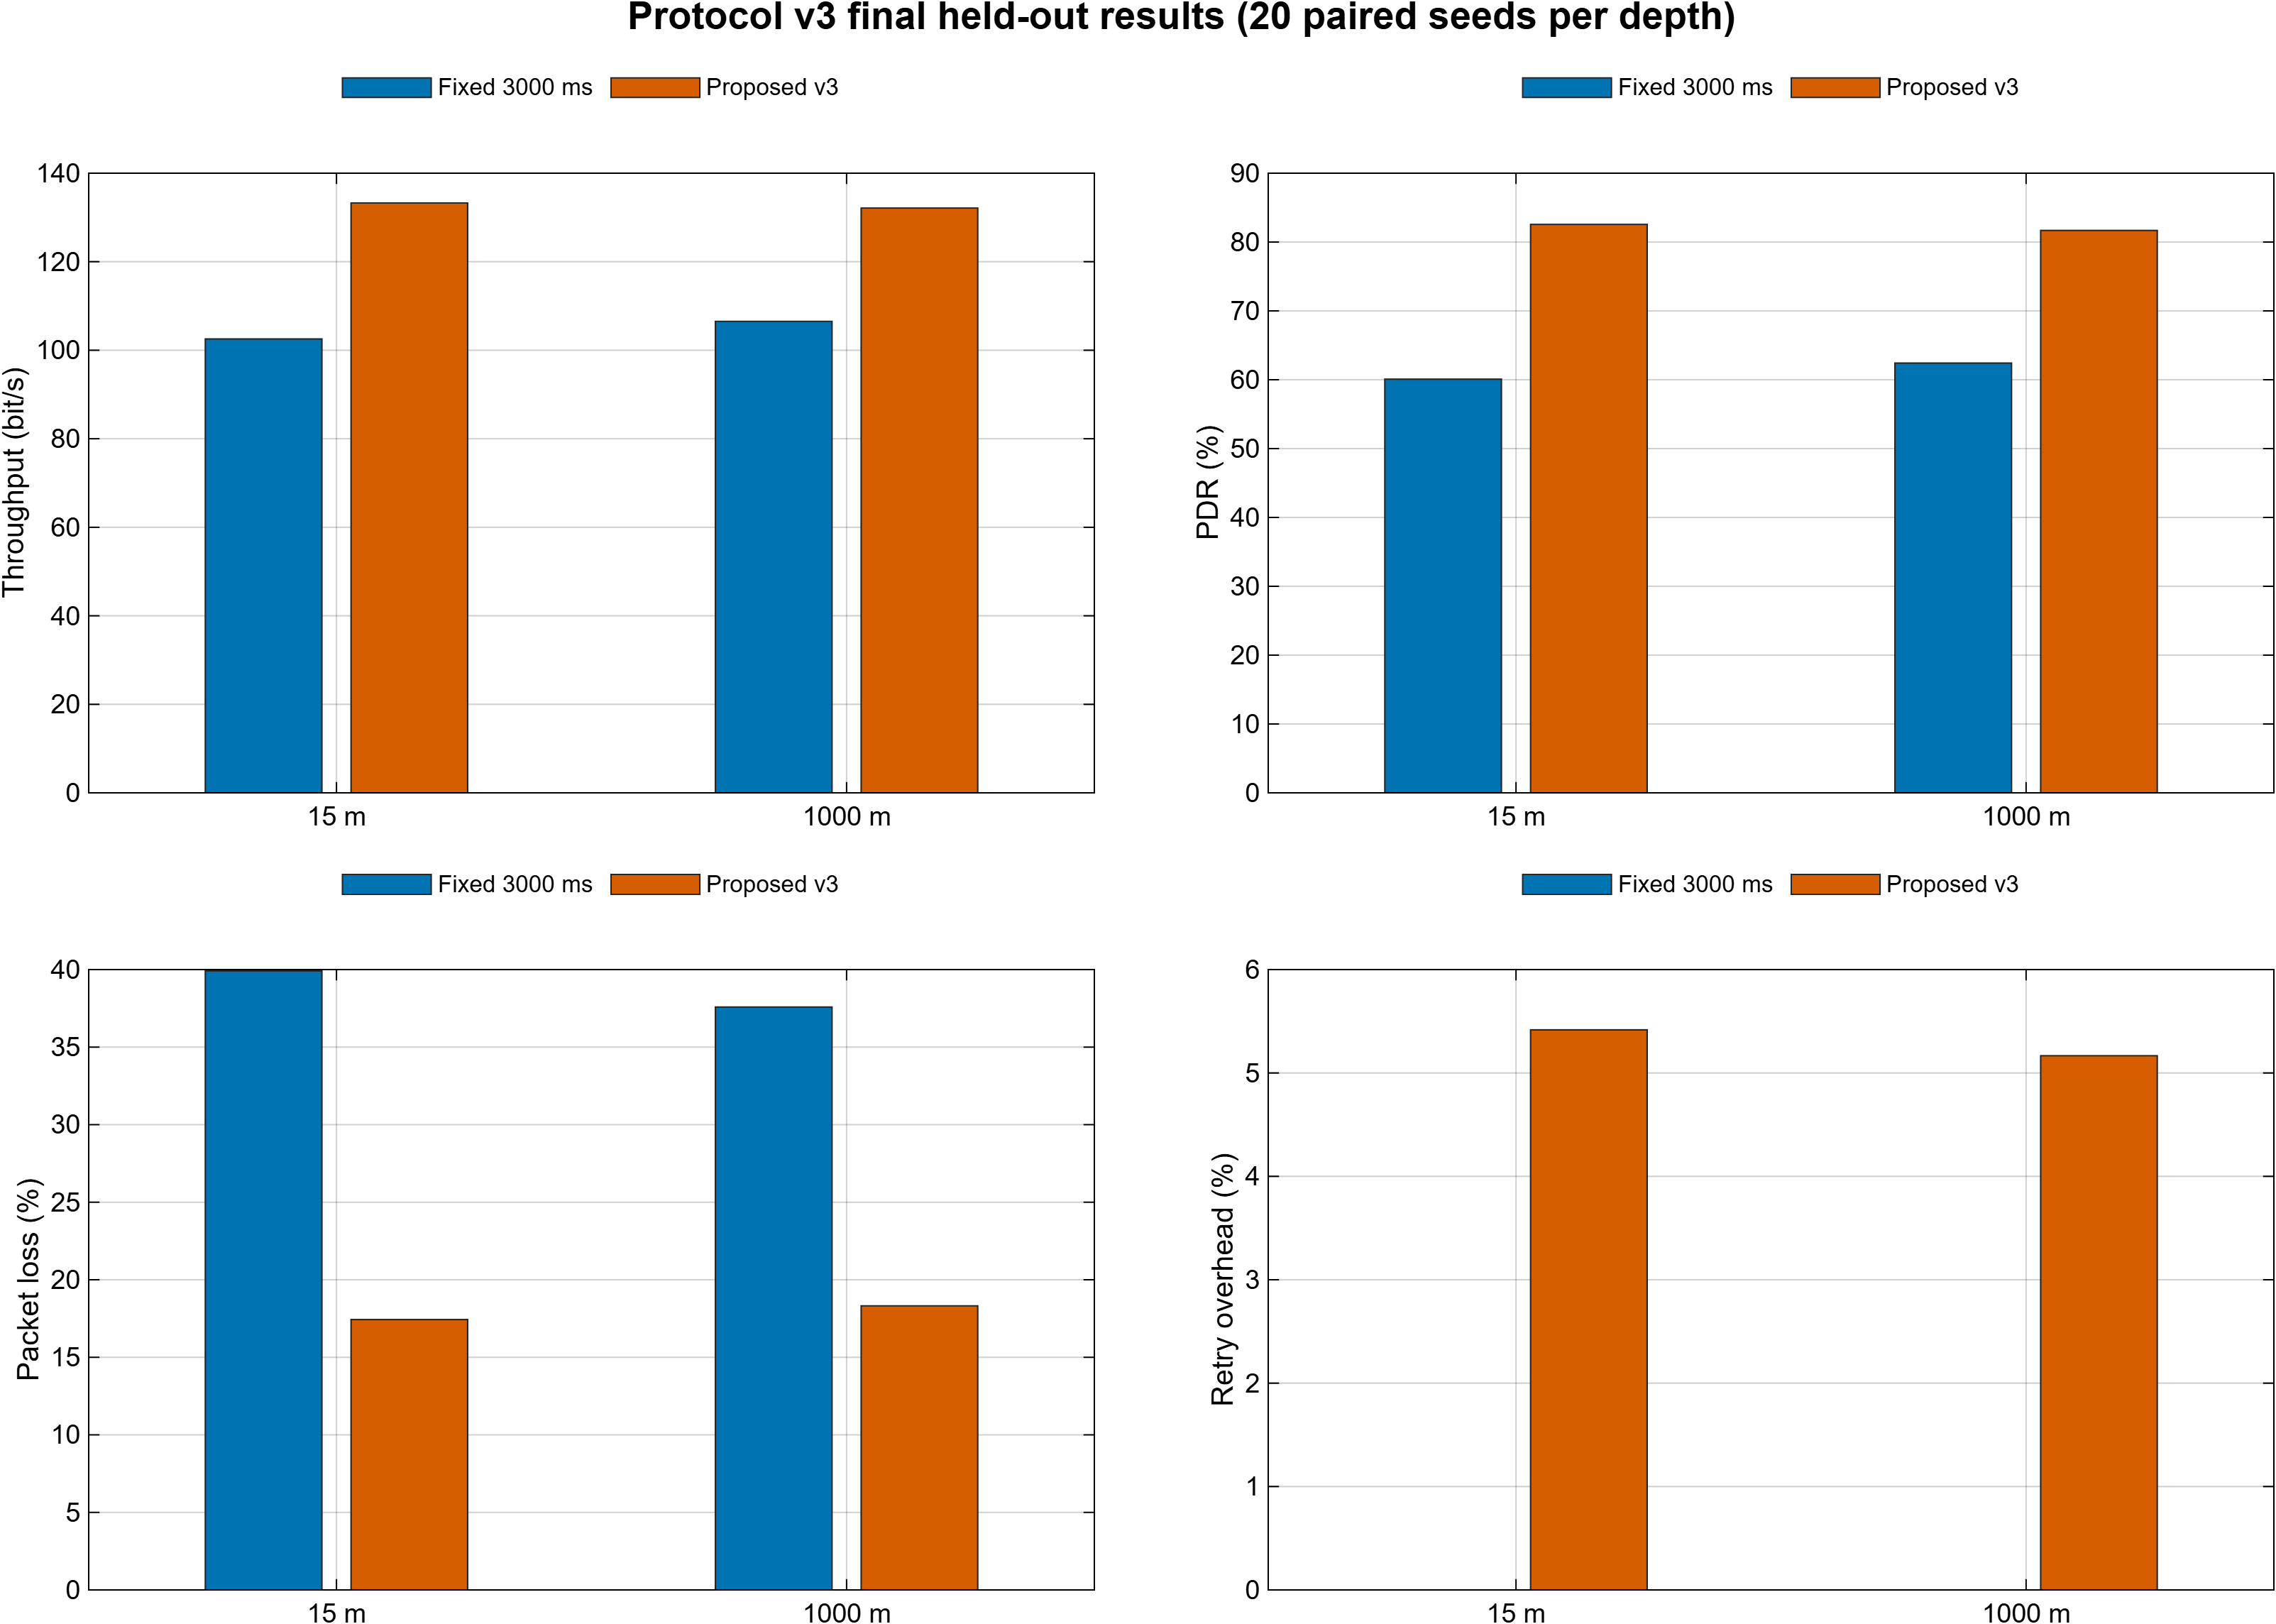
\includegraphics[width=0.92\linewidth]{images/final_dashboard.png}
\caption{Final Protocol~v3 dashboard from the validated held-out summary files.}\label{fig:dashboard}
\end{figure}

\subsection{Useful throughput}\label{sec:res-throughput}
\noindent
At 15~m, Protocol~v3 delivered 46.85 unique messages per run.
Fixed mode delivered 36.05.
Useful throughput increased from 102.54 to 133.26~bit/s.
The paired increase was 30.63\%.

At 1000~m, Protocol~v3 delivered 46.45 unique messages per run.
Fixed mode delivered 37.45.
Useful throughput increased from 106.52 to 132.12~bit/s.
The paired increase was 24.30\%.

\begin{figure}[H]
\centering
\begin{minipage}[t]{0.49\linewidth}
\centering
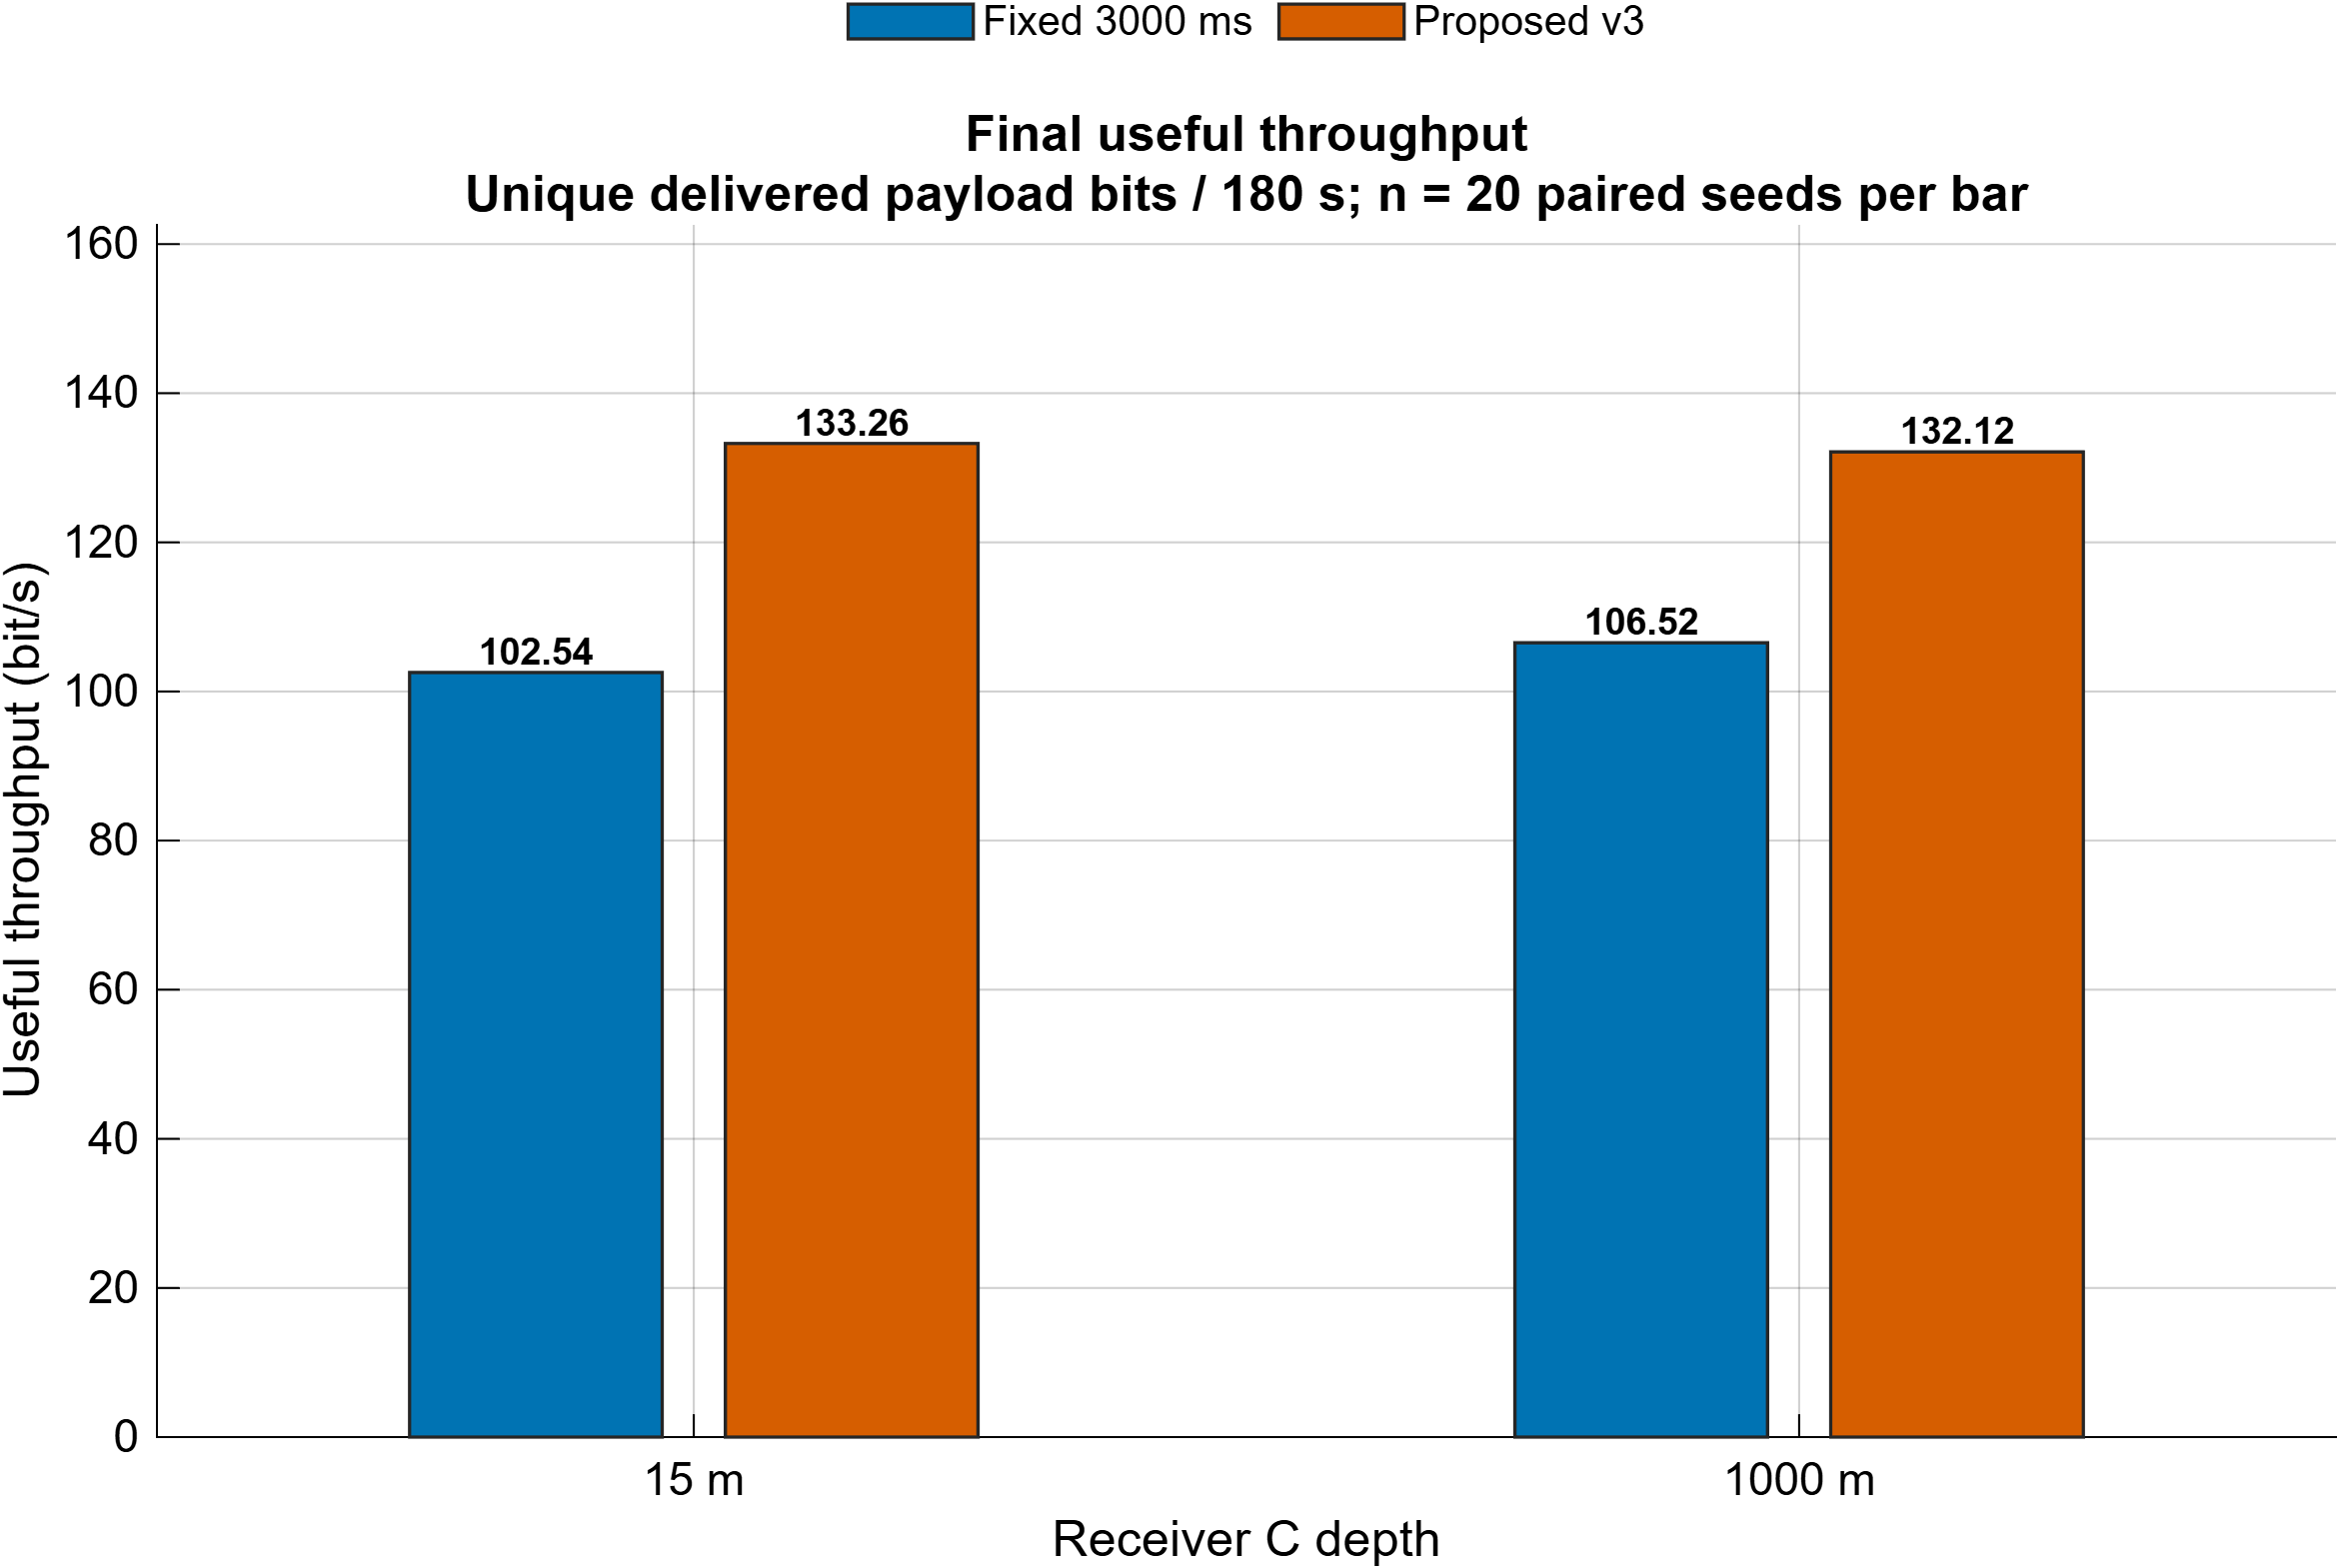
\includegraphics[width=\linewidth]{images/throughput.png}
\caption{Mean useful throughput.}\label{fig:throughput}
\end{minipage}\hfill
\begin{minipage}[t]{0.49\linewidth}
\centering
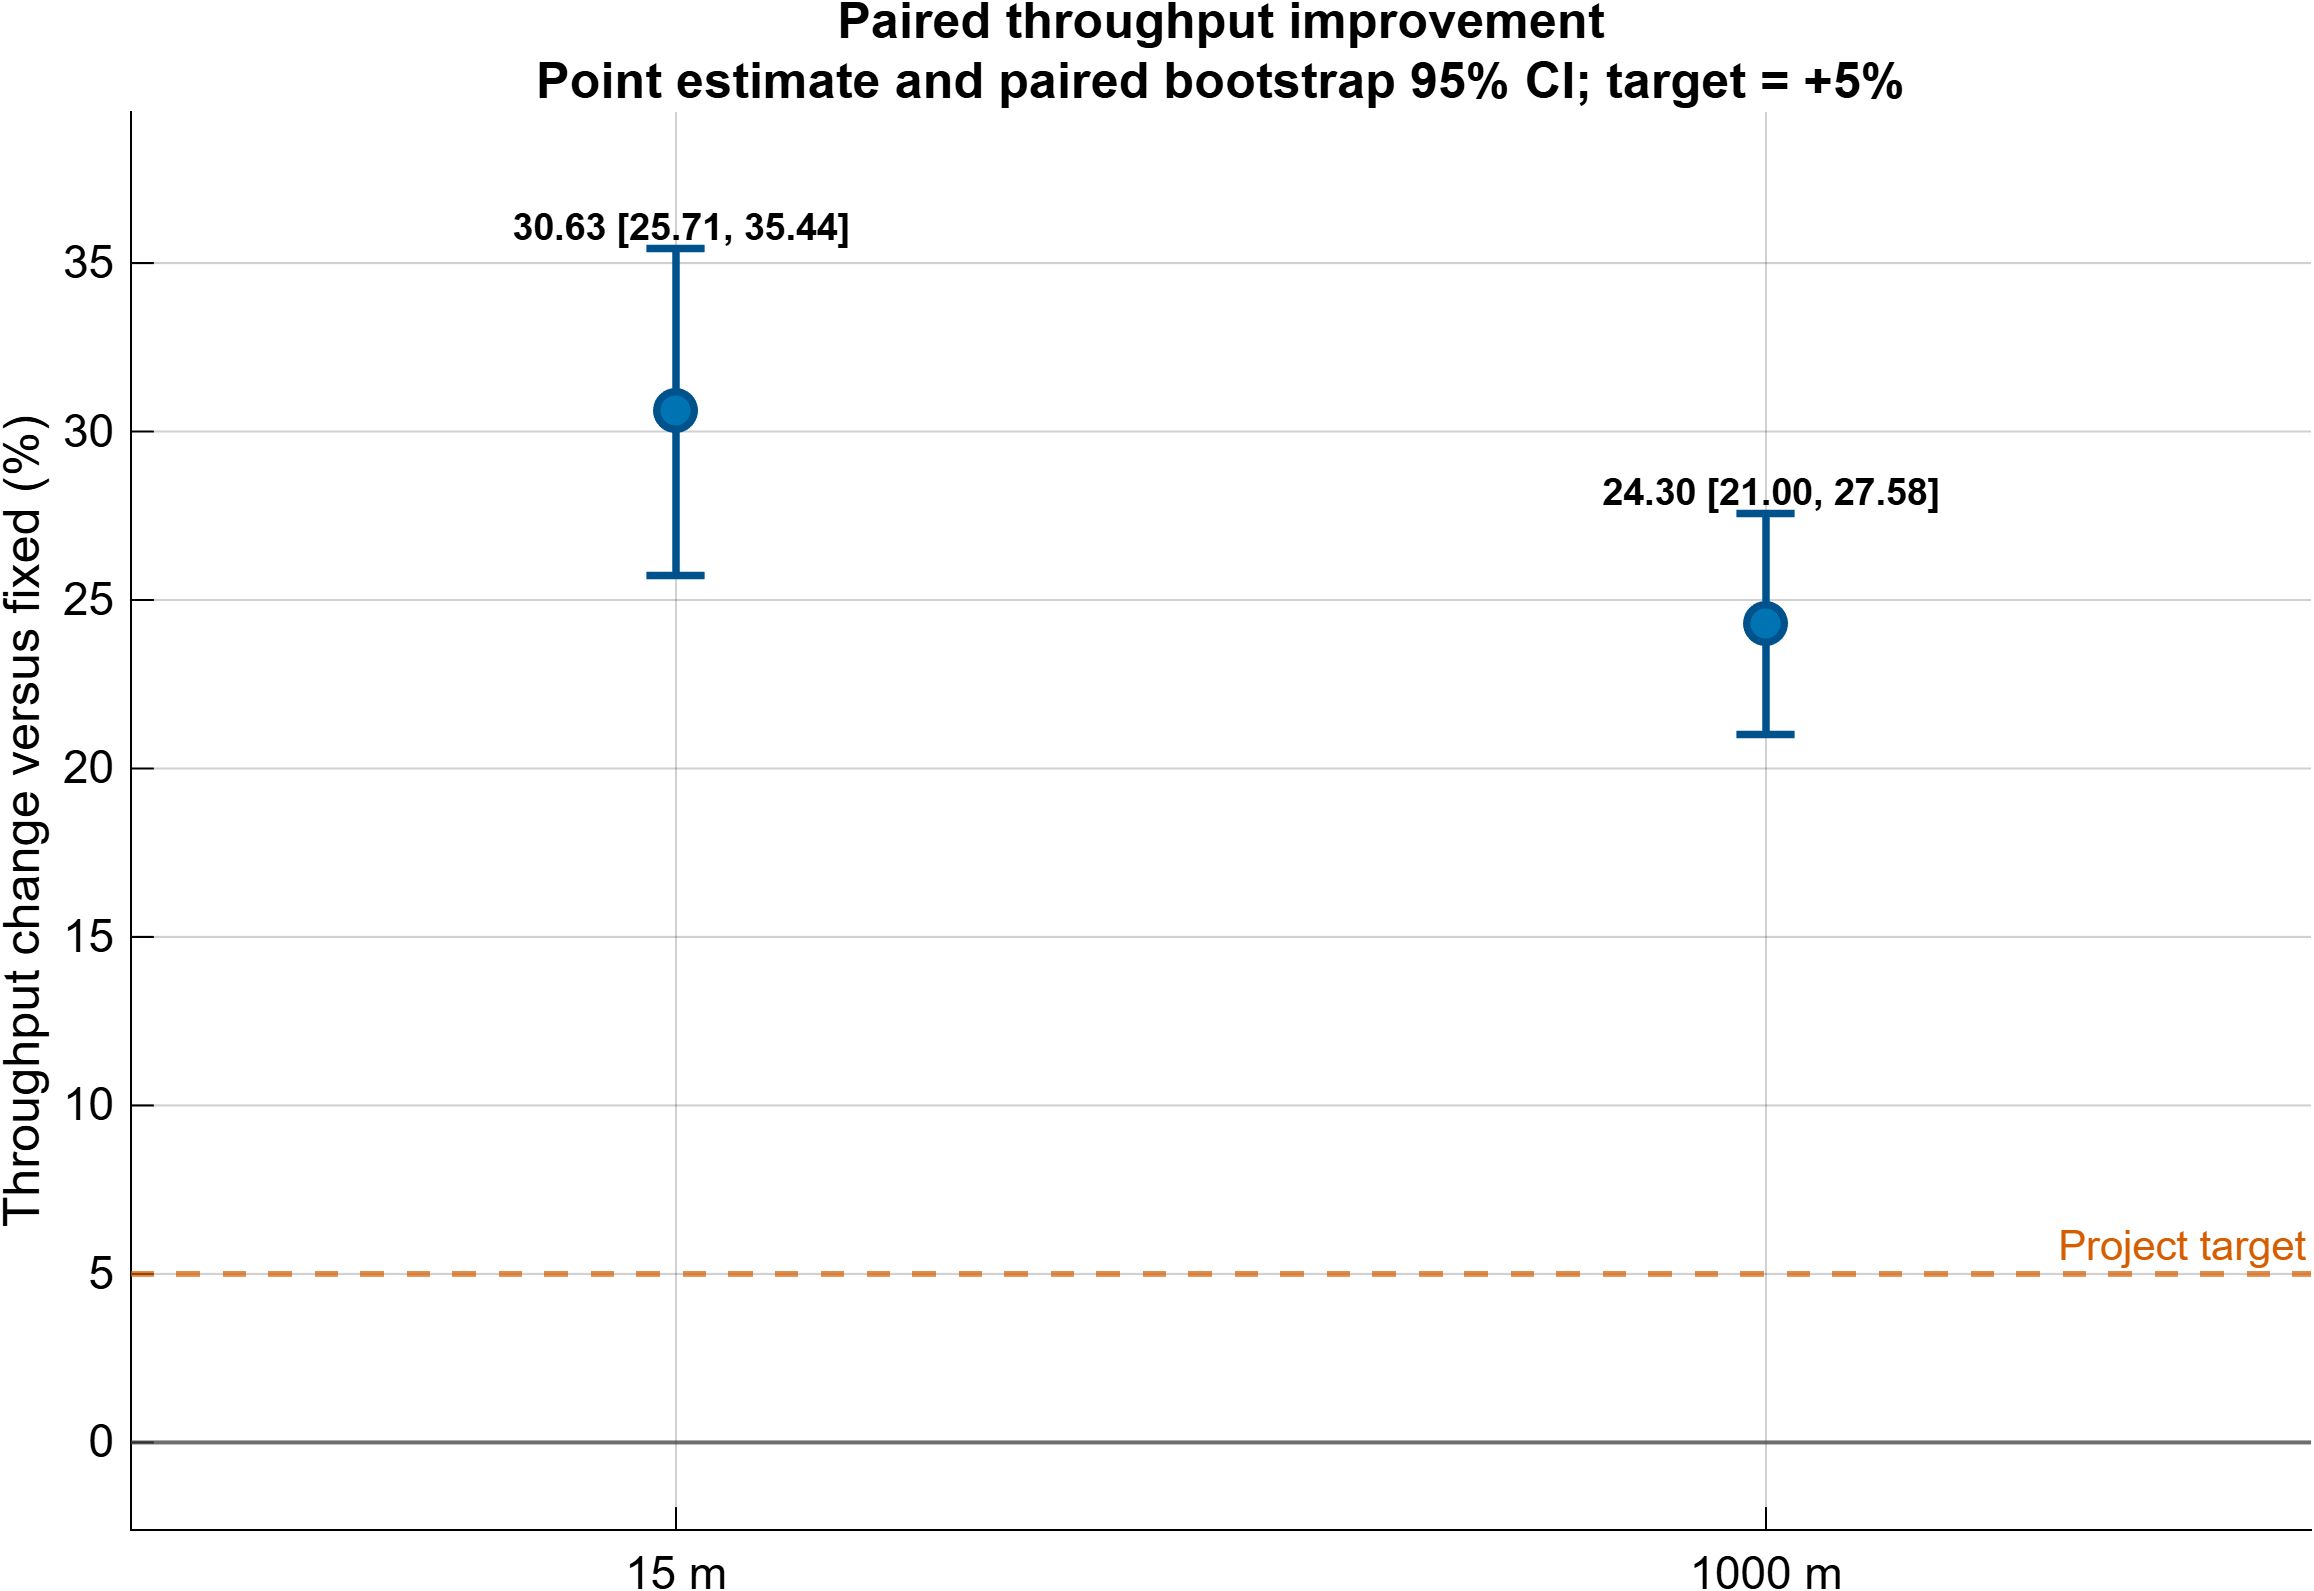
\includegraphics[width=\linewidth]{images/throughput_gain.png}
\caption{Paired throughput gain and 95\% intervals.}\label{fig:throughput-gain}
\end{minipage}
\end{figure}

\subsection{Packet delivery and confirmed loss}\label{sec:res-pdr}
\noindent
At 15~m, PDR increased from 60.08\% to 82.57\%.
The paired change was 22.48 percentage points.
At 1000~m, PDR increased from 62.42\% to 81.68\%.
The paired change was 19.26 percentage points.

\begin{figure}[H]
\centering
\begin{minipage}[t]{0.49\linewidth}
\centering
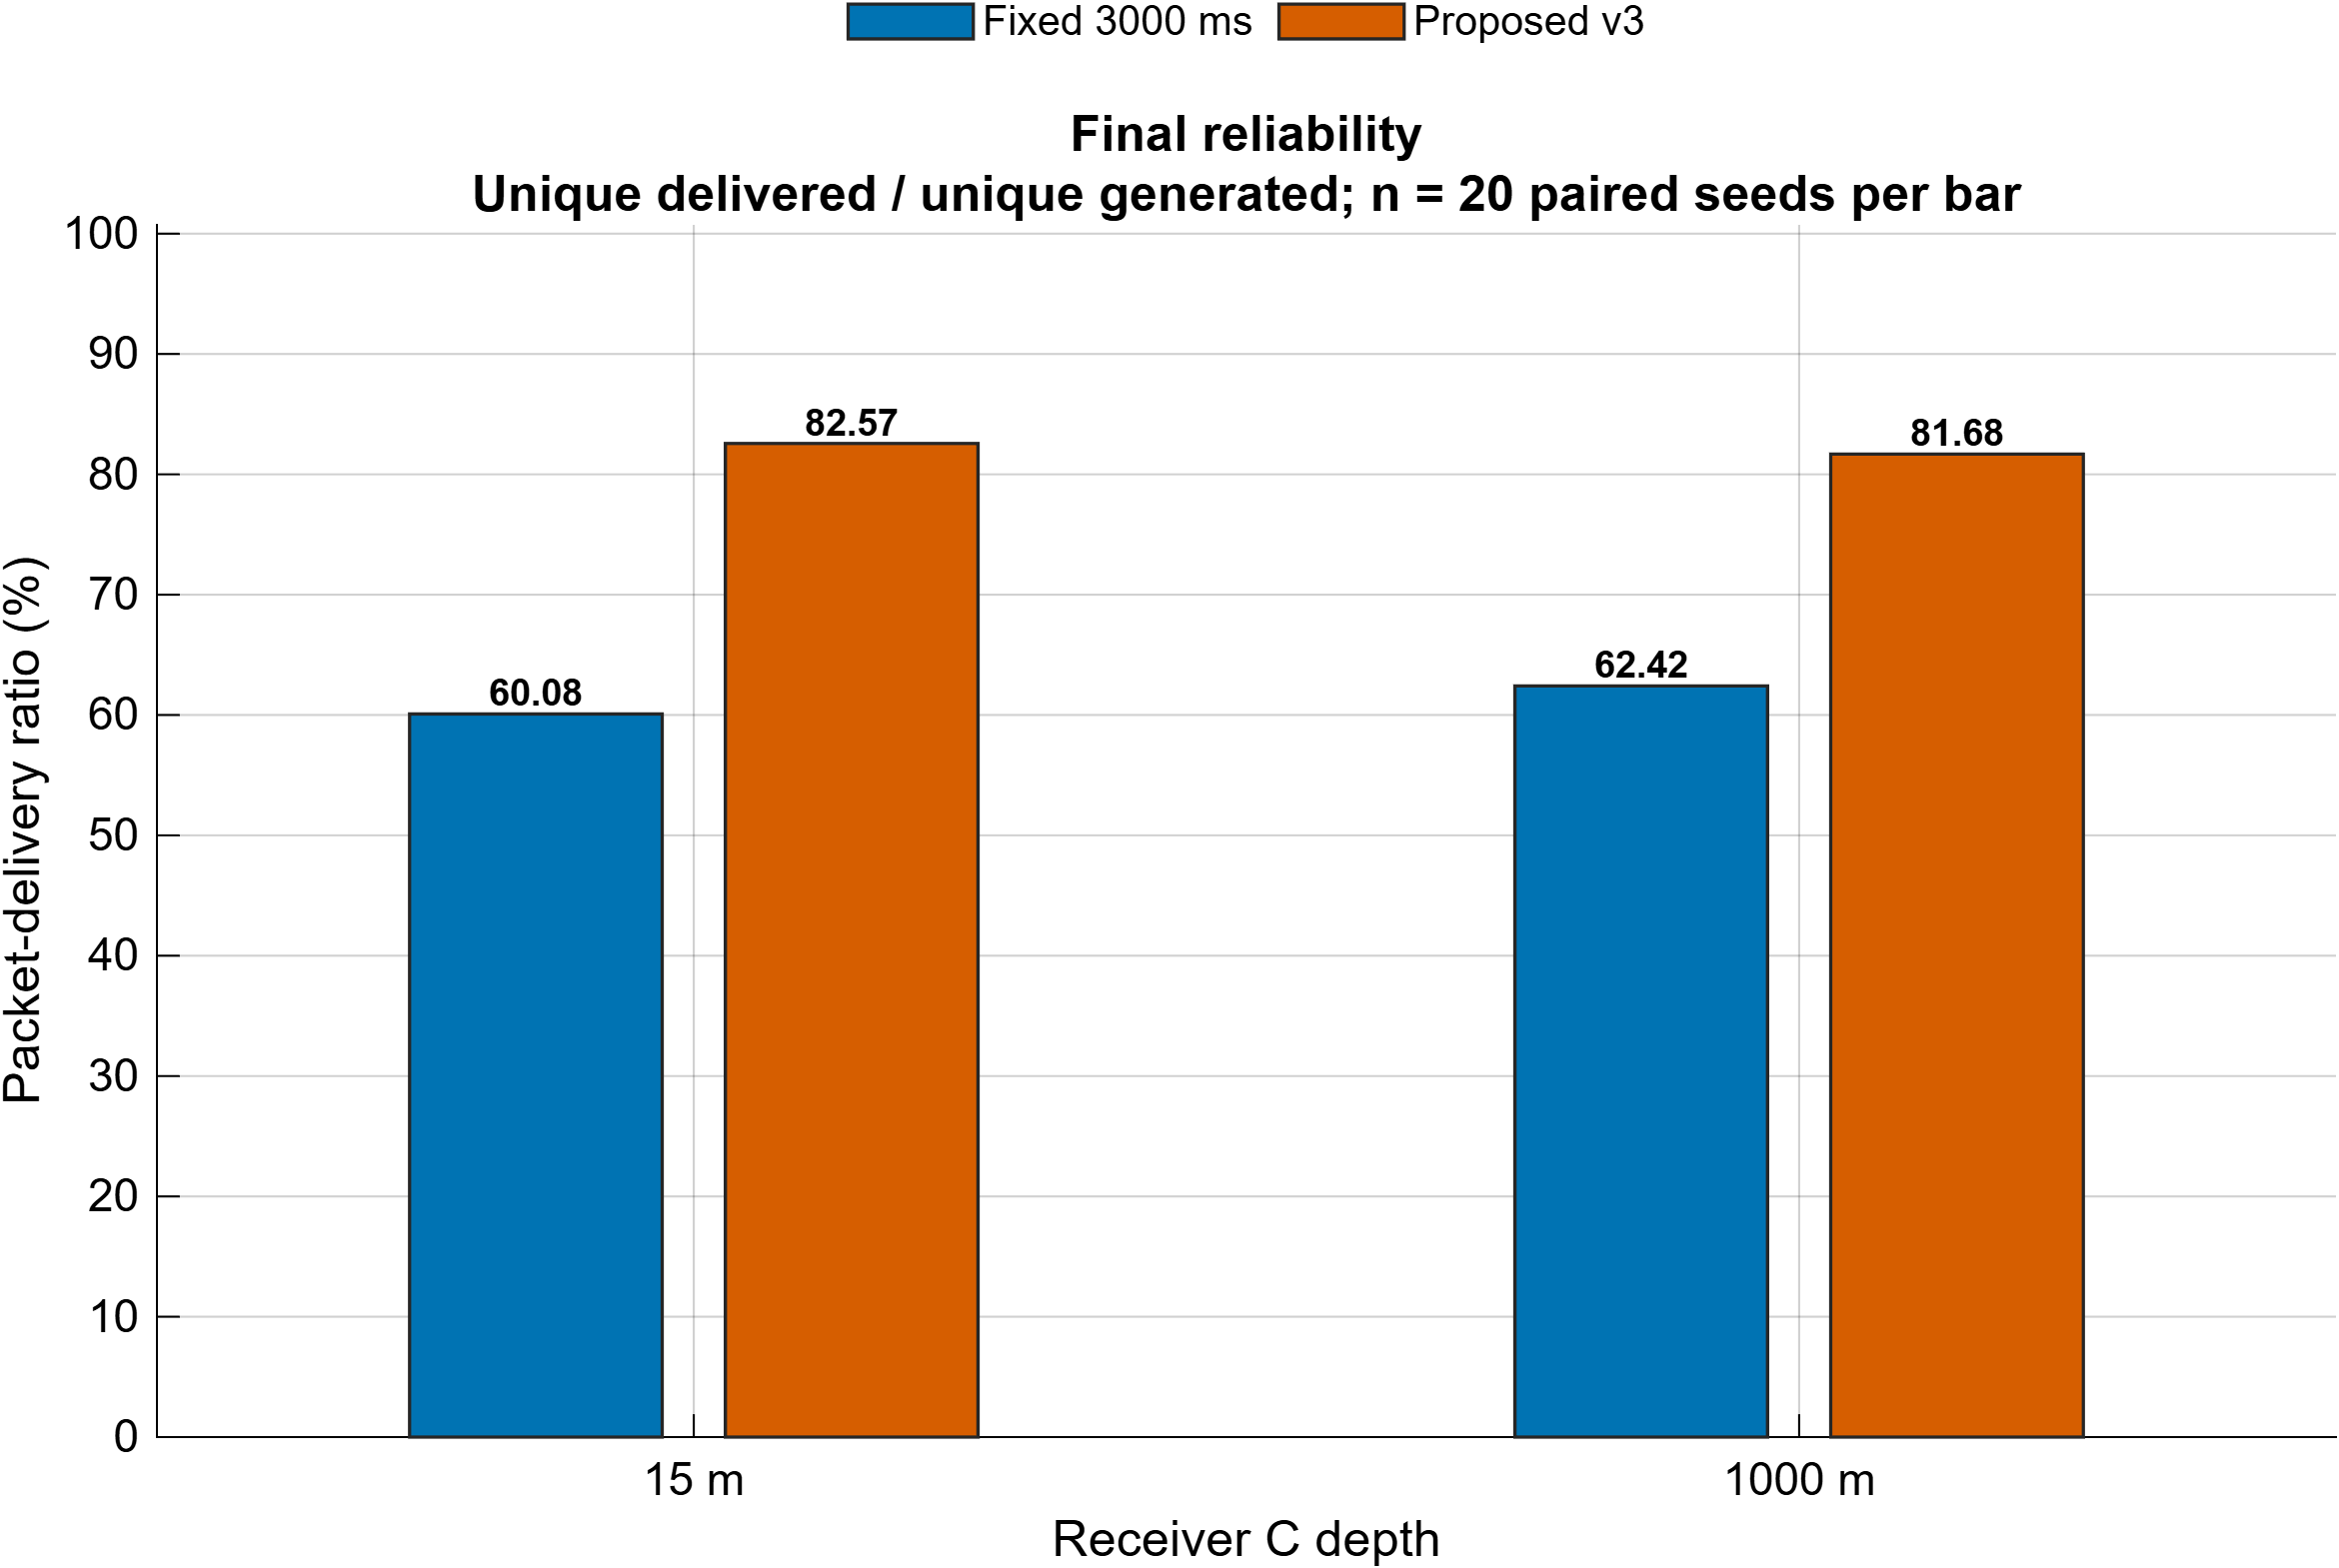
\includegraphics[width=\linewidth]{images/pdr.png}
\caption{Packet-delivery ratio.}\label{fig:pdr}
\end{minipage}\hfill
\begin{minipage}[t]{0.49\linewidth}
\centering
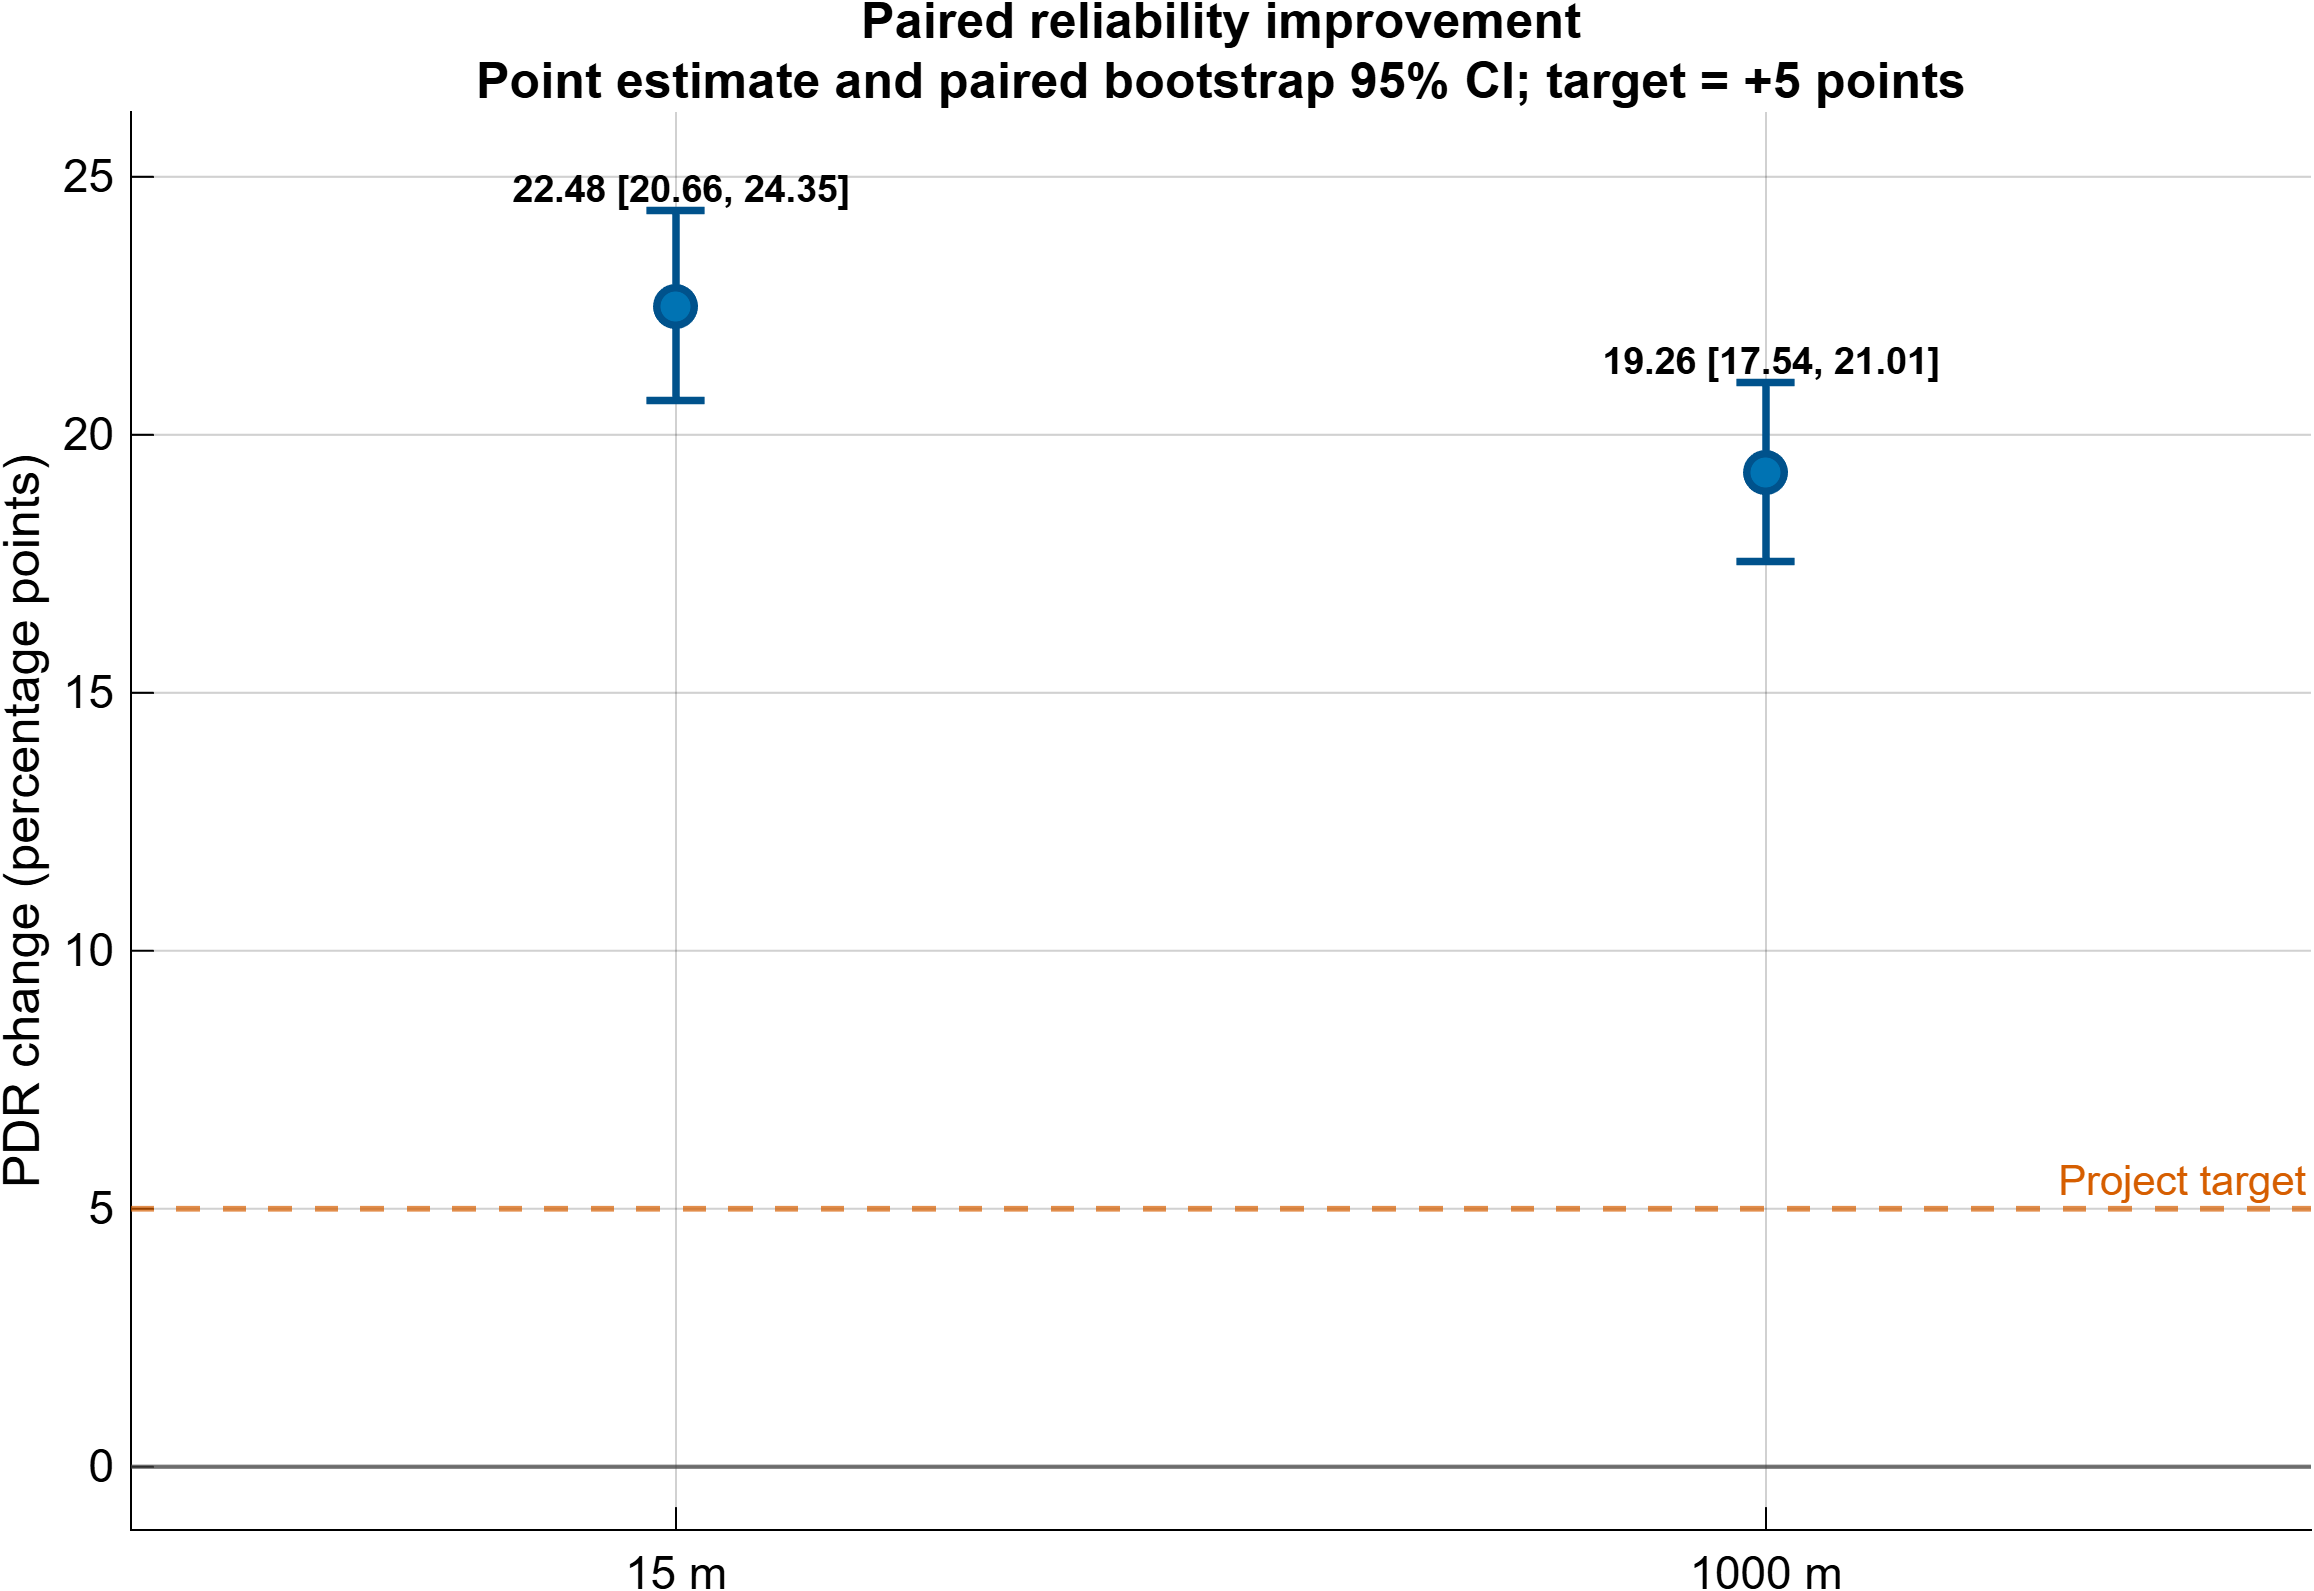
\includegraphics[width=\linewidth]{images/pdr_gain.png}
\caption{Paired PDR gain and 95\% intervals.}\label{fig:pdr-gain}
\end{minipage}
\end{figure}

\subsection{Retry and RTT diagnostics}\label{sec:res-diagnostics}
\noindent
Protocol~v3 used 5.42\% retry overhead at 15~m and 5.17\% at 1000~m.
The retry scheduler kept recovery bounded.
Fixed mode used no application-layer retry.

RTT is a diagnostic metric in this comparison.
Fixed mode requests an ACK for each original.
Protocol~v3 requests two original ACKs per full window and an ACK for each retry.
The two protocols therefore sample different ACK populations.
RTT alone is not the reliability claim.

\begin{figure}[H]
\centering
\begin{minipage}[t]{0.49\linewidth}
\centering
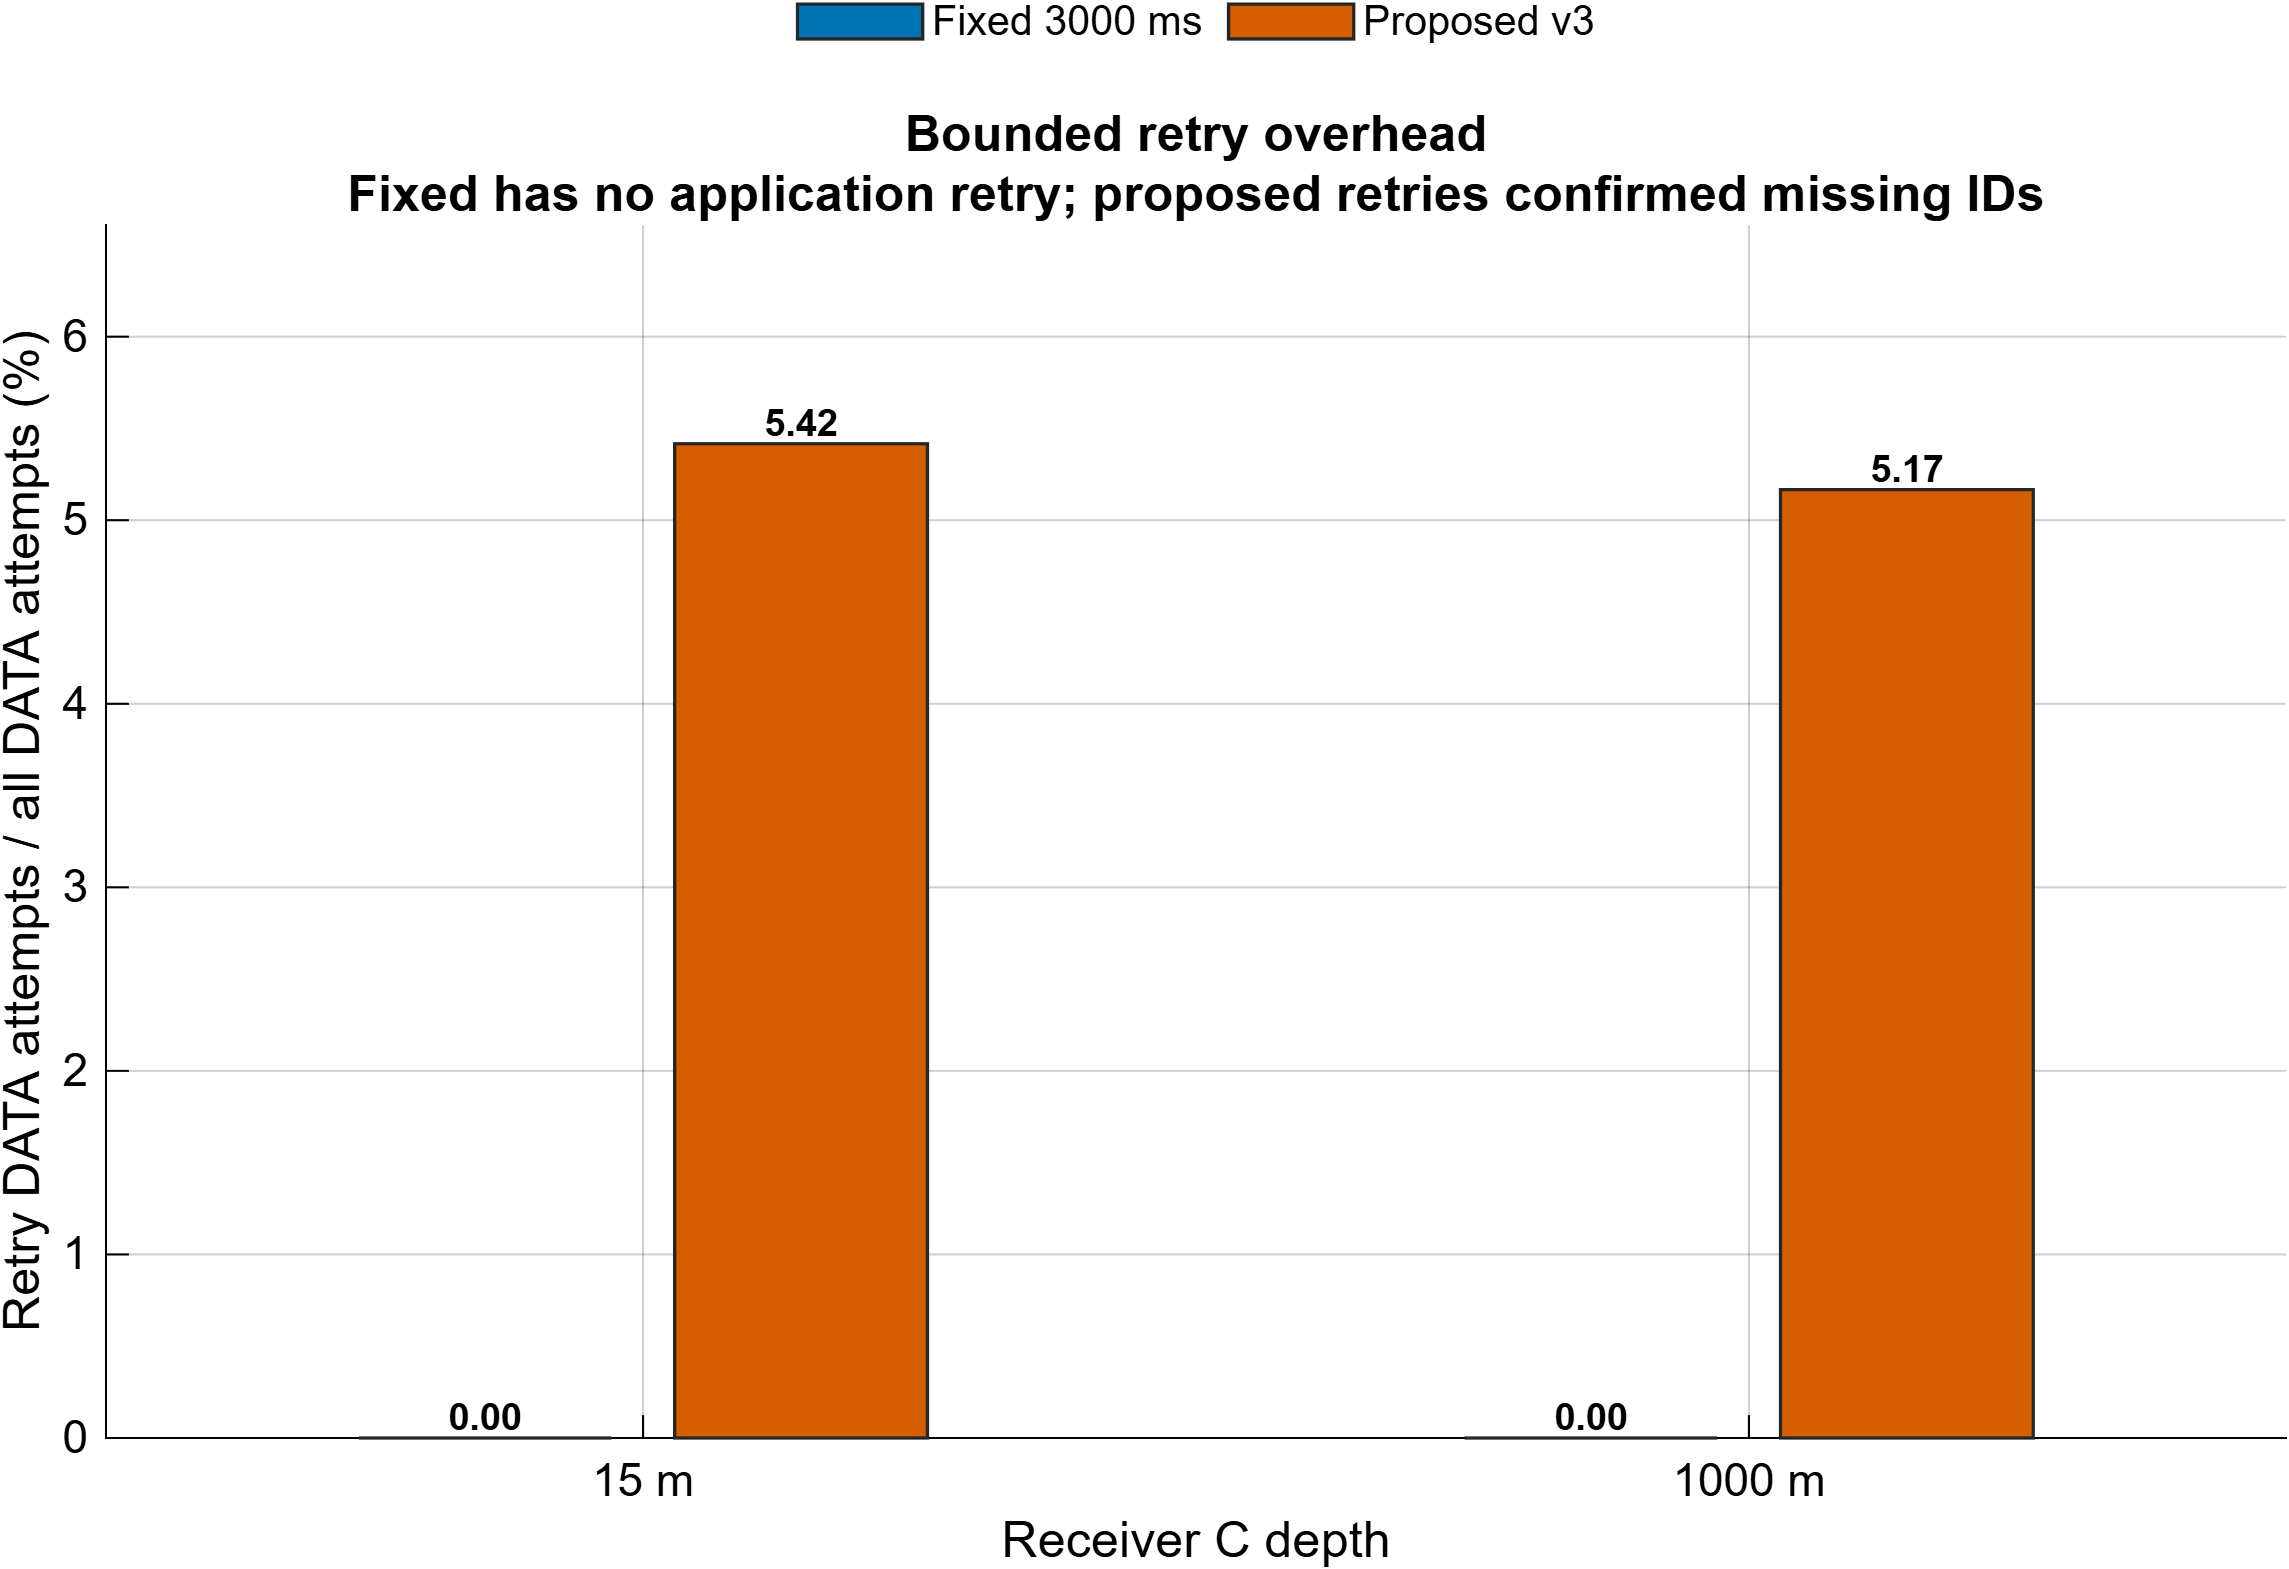
\includegraphics[width=\linewidth]{images/retry_overhead.png}
\caption{Bounded retry overhead.}\label{fig:retry-overhead}
\end{minipage}\hfill
\begin{minipage}[t]{0.49\linewidth}
\centering
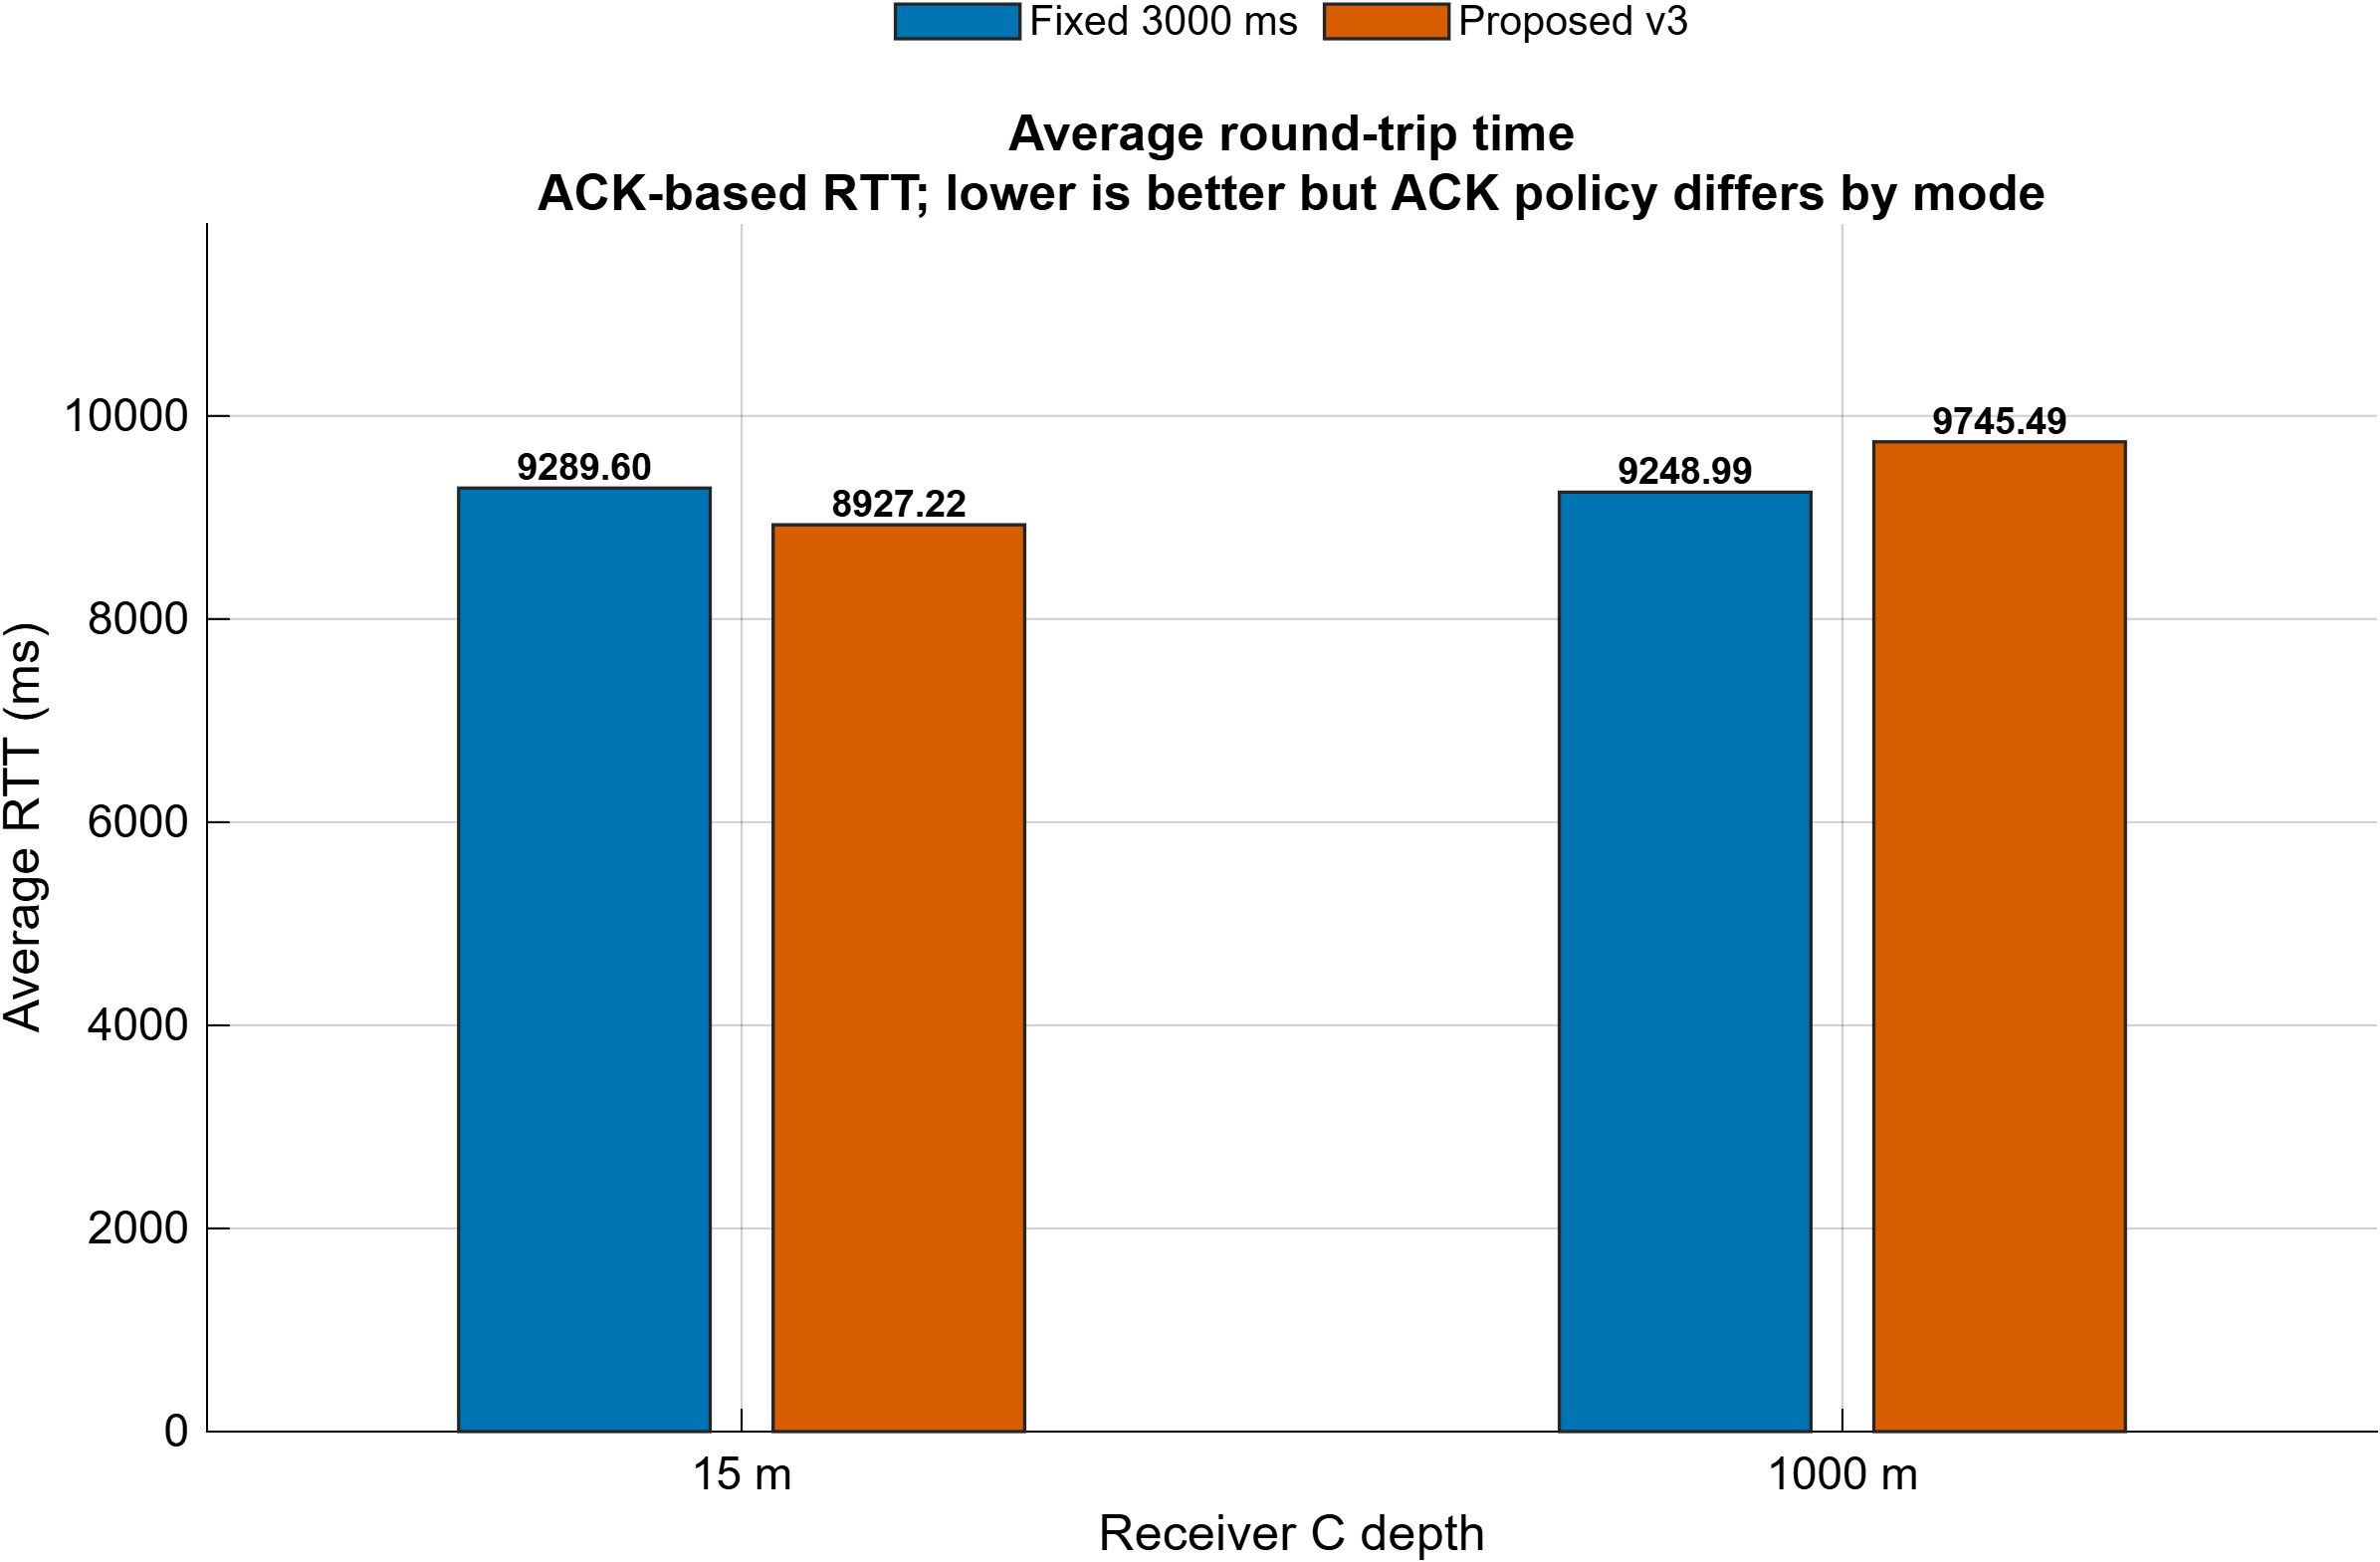
\includegraphics[width=\linewidth]{images/average_rtt.png}
\caption{Mean RTT for each protocol's ACK samples.}\label{fig:rtt}
\end{minipage}
\end{figure}

\subsection{Effect of depth}\label{sec:res-depth}
\noindent
Depth does not have a general rule that makes throughput increase.
A depth change can change 3D distance, propagation delay, and collision timing.
It does not automatically improve channel quality.
The moderate detection and decoding probabilities stay equal at both depths in this experiment.

\begin{table}[H]
\centering\small
\caption{Paired throughput effect of moving receiver C from 15~m to 1000~m.}\label{tab:depth}
\begin{tabular}{l c c p{5.6cm}}
\toprule
Mode & Change & 95\% interval & Result \\
\midrule
Fixed & +3.98~bit/s & +0.57 to +7.82 & Positive in this fixed-mode experiment \\
Protocol~v3 & $-1.14$~bit/s & $-3.56$ to +1.42 & Inconclusive because the interval includes zero \\
\bottomrule
\end{tabular}
\end{table}

\begin{figure}[H]
\centering
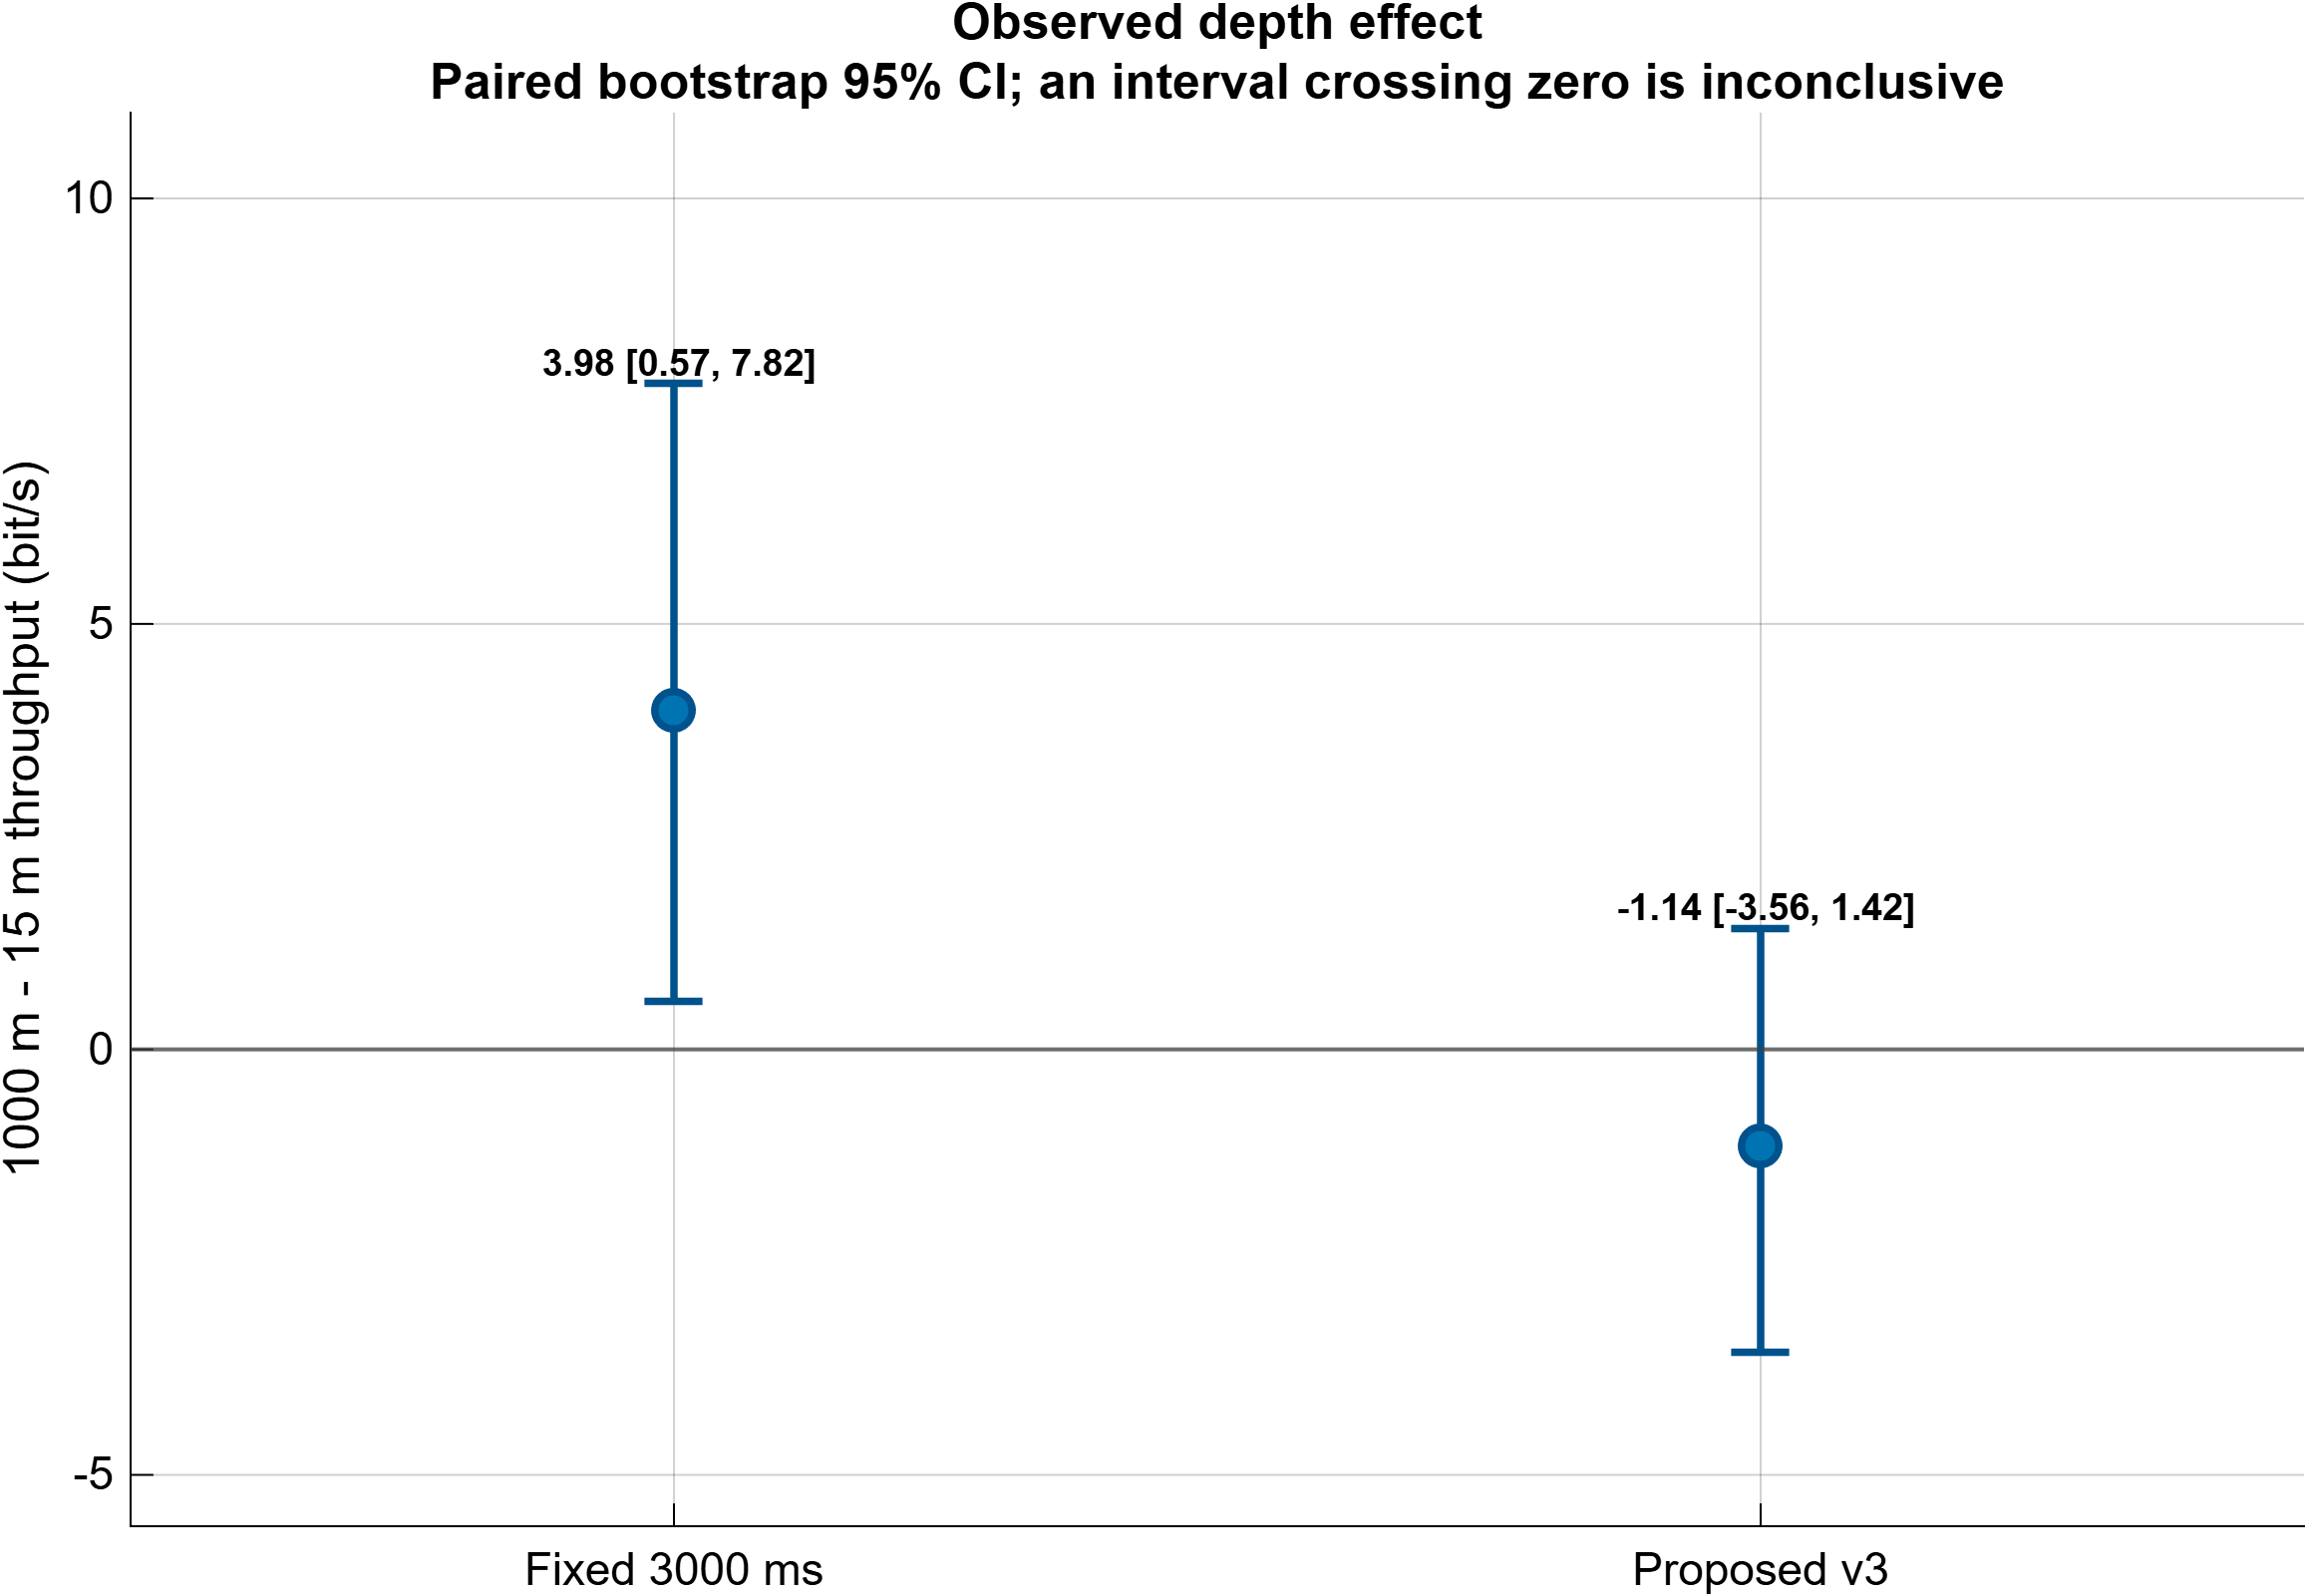
\includegraphics[width=0.86\linewidth]{images/depth_effect.png}
\caption{Paired effect of the receiver-depth change on useful throughput.}\label{fig:depth}
\end{figure}

The correct conclusion is limited.
Fixed throughput increased in this simulation.
Protocol~v3 did not show a supported depth increase.
The experiment does not support the statement that throughput always increases when depth increases.

\subsection{Comparison with the state of the art}\label{sec:res-sota}
\noindent
The numerical comparison is between fixed mode and Protocol~v3.
We did not reimplement the other literature methods.
Table~\ref{tab:sota} therefore compares their mechanisms and reported objectives, not their numerical results.

\begin{table}[H]
\centering\footnotesize\setlength{\tabcolsep}{3pt}
\caption{Mechanism comparison with the reviewed approaches.}\label{tab:sota}
\begin{tabular}{>{\raggedright\arraybackslash}p{2.7cm} >{\raggedright\arraybackslash}p{3.4cm} >{\raggedright\arraybackslash}p{3.6cm} >{\raggedright\arraybackslash}p{3.4cm} >{\raggedright\arraybackslash}p{2.1cm}}
\toprule
Method & Rate or schedule decision & Feedback load & Recovery & This experiment \\
\midrule
Fixed baseline & No rate change & ACK for each original & None & Measured \\
Multi-hop ARQ~\cite{tan2007} & Stop-and-wait state & ACK based & Retransmission & Not reimplemented \\
ATC~\cite{guo2008} & BER and topology schedule & Periodic link feedback & Collision reduction & Not reimplemented \\
Protocol~v3 & Receiver-validated weighted score & 2 original ACKs per 10-message window & Bounded selective retry & Measured \\
\bottomrule
\end{tabular}
\end{table}

Protocol~v3 produced 82.57\% PDR at 15~m and 81.68\% at 1000~m.
Fixed mode produced 60.08\% and 62.42\%.
This comparison supports the improvement over the declared baseline.
It does not prove a numerical advantage over ARQ or ATC under their original settings.

\subsection{Limitations}\label{sec:res-limits}
\begin{enumerate}\setlength{\itemsep}{2pt}
  \item The experiment uses a three-node simulated topology.
  \item The moderate scenario uses fixed detection and decoding probabilities.
  \item The model does not use a measured sound-speed profile, salinity profile, or thermocline.
  \item The experiment uses two receiver depths and one horizontal geometry.
  \item The evidence comes from simulation, not a sea trial.
  \item RTT and timeout samples differ because the ACK policies differ.
  \item Protocol~v3 needs receiver-report state and more application logic than fixed mode.
\end{enumerate}

\subsection{Reproducibility}\label{sec:res-reproducibility}
\noindent
The repository contains the simulation scripts, controller code, tests, frozen configuration, 80 held-out run directories, summary CSV files, and MATLAB graph script.
The run matrix uses seeds 211--230 for held-out evaluation.
The analyzer checks protocol version, mode, depth, seed, measurement time, manifest status, and node event files before it accepts a run.

%==========================================================
\section{Conclusions and future work}\label{sec:conclusion}
\noindent
The purpose of this work was to improve useful data delivery in an underwater acoustic network without changing the modem data rate.
The fixed baseline used a 3000~ms application sending interval, one acknowledgment request for each original message, and no application-layer retry.
Protocol~v3 used sparse acknowledgments, immutable receiver snapshots, a weighted network-condition score, and bounded selective retry.
We implemented both protocols in UnetStack~7.0.0.
Python validated the runs and calculated paired effects.
MATLAB recreated the final graphs from validated CSV files.

The held-out evaluation used 20 paired seeds at each of two depths.
Protocol~v3 increased useful throughput by 30.63\% at 15~m and 24.30\% at 1000~m.
It increased packet-delivery ratio by 22.48 and 19.26 percentage points.
All four paired 95\% intervals excluded zero.
Retry overhead was 5.42\% and 5.17\%.
The results meet the project target for the declared simulation.
They do not show that depth always increases throughput.

Future work must test larger and mobile topologies.
It must use measured channel traces and more channel states.
A field test must run the same protocol on compatible UnetStack modem hardware.
Future tests must also measure energy use and control-byte cost.

%==========================================================
\begin{thebibliography}{99}
\small

\bibitem{akyildiz2005}
I. F. Akyildiz, D. Pompili, and T. Melodia, ``Underwater acoustic sensor networks: Research challenges,'' \emph{Ad Hoc Networks}, vol.~3, no.~3, pp.~257--279, 2005, doi: 10.1016/j.adhoc.2005.01.004.

\bibitem{tan2007}
H.-P. Tan, W. K. G. Seah, and L. Doyle, ``A multi-hop ARQ protocol for underwater acoustic networks,'' in \emph{Proc. OCEANS 2007 Europe}, 2007, pp.~1--6, doi: 10.1109/OCEANSE.2007.4302195.

\bibitem{guo2008}
Z.-W. Guo, X.-D. Liu, and Y. Feng, ``An adaptive transmission control mechanism for underwater acoustic sensor network,'' in \emph{Proc. IFIP Int. Conf. Network and Parallel Computing}, 2008, doi: 10.1109/NPC.2008.33.

\bibitem{casari2011}
P. Casari and M. Zorzi, ``Protocol design issues in underwater acoustic networks,'' \emph{Computer Communications}, vol.~34, no.~17, pp.~2013--2025, 2011, doi: 10.1016/j.comcom.2011.06.008.

\bibitem{chitre2014}
M. Chitre, R. Bhatnagar, and W.-S. Soh, ``UnetStack: An agent-based software stack and simulator for underwater networks,'' in \emph{Proc. OCEANS 2014}, 2014, pp.~1--10, doi: 10.1109/OCEANS.2014.7003044.

\bibitem{unethandbook}
UnetStack, ``Unet handbook: Simulating networks.'' [Online]. Available: \url{https://unetstack.net/handbook/402_sim.html}. Accessed: Nov. 2, 2026.

\bibitem{asdste100}
ASD Simplified Technical English Maintenance Group, ``ASD-STE100 Simplified Technical English, Issue~9,'' Jan. 15, 2025. [Online]. Available: \url{https://www.asd-ste100.org/assets/files/ASD-STE100_ISSUE9.pdf}.

\bibitem{kassis2026}
T. Kassis, V. Agarwal, Y. He, D. Patel, and A. M. Brueckner, ``Scientific Agent Skills: A library of procedural knowledge for research agents,'' \emph{arXiv preprint arXiv:2609.00065}, 2026, doi: 10.48550/arXiv.2609.00065.

\end{thebibliography}

\end{document}
